\documentclass[12pt]{article}
\usepackage{bookmark}
% --- Paquetes para el diseño ---
\usepackage[utf8]{inputenc}
\usepackage{lmodern}
\usepackage[spanish,provide=*]{babel}
\usepackage[margin=1.5cm,top=2cm, bottom=3cm,headheight=0pt, headsep=0.5cm]{geometry}
\usepackage{graphicx}
\usepackage{float}
\usepackage{xcolor}
\usepackage{tcolorbox} % Para los cuadros grises redondeados
\tcbuselibrary{breakable}
\usepackage{array}
\usepackage{hyperref}
\setkeys{Hyp}{breaklinks=true} % Fuerza a hyperref a romper los enlaces largos
\urlstyle{same}                % Opcional: Hace que la fuente de la URL sea igual a la del texto
\usepackage{fancyhdr}   % Para el encabezado de las páginas siguientes
\usepackage{titlesec}   % Para personalizar los títulos
\usepackage{enumitem}
\usepackage{listings}
\usepackage{caption}
\usepackage{amssymb} % Necesario para los símbolos N y Z
\usepackage{amsmath} % Recomendado para texto dentro de fórmulas
\usepackage{algorithm}
\usepackage{algpseudocode}
\usepackage{setspace}

\renewcommand{\baselinestretch}{1.1} % 1.3 equivale aproximadamente a un interlineado de 1.5

% Configuración para quitar "Listing #:"
\DeclareCaptionFormat{listing}{\textbf{#3}}

% --- ESTILO PARA C (Multihilos) ---
\lstdefinestyle{estiloC}{
    language=C,
    basicstyle=\ttfamily\small,
    keywordstyle=\color{blue}\bfseries,
    commentstyle=\color{green!50!black},
    stringstyle=\color{orange},
    numbers=left,
    numberstyle=\tiny\color{green!50!black},
    stepnumber=1,
    numbersep=8pt,
    frame=single,
    rulecolor=\color{black},
    breaklines=true,
    showstringspaces=false,
    tabsize=4,
    keepspaces=true,
    columns=flexible,
    xleftmargin=20pt,
    morekeywords={NULL, sendto, recvfrom, bzero, printf, close, exit, perror, strlen, memset, memcpy, bind, typedef, struct, pthread_create, pthread_join, sleep, usleep, read, rand, srand, strcmp, sprintf, write, Mensaje, Info, nodoP2P, colaP2P, tiempo, p2p, hilo_escucha, wait, enviar_msj, getpid, fclose, fprintf, snprintf, fopen, FILE, setsockopt, AF_INET, SOCK_DGRAM, INADDR_ANY, htons, inet_pton, socket, listen, accept, send, connect, convertir_hora, convertion_ms, convertir_tiempo, capturar_tiempo, encolarP2P, desencolarP2P, free},
    extendedchars=true,
    % Se añaden los signos de exclamación e interrogación invertidos:
    literate={á}{{\'a}}1 {é}{{\'e}}1 {í}{{\'i}}1 {ó}{{\'o}}1 {ú}{{\'u}}1 {ñ}{{\~n}}1
             {Á}{{\'A}}1 {É}{{\'E}}1 {Í}{{\'I}}1 {Ó}{{\'O}}1 {Ú}{{\'U}}1 {Ñ}{{\~N}}1
             {¡}{{\exclamdown}}1 {¿}{{\questiondown}}1
}

\lstdefinestyle{estiloPseudo}{
    language={}, % Se deja vacío para que no use las palabras clave de C
    basicstyle=\ttfamily\small,
    keywordstyle=\color{purple}\bfseries, % Color distintivo para palabras clave
    commentstyle=\color{gray}\itshape,    % Comentarios en gris e itálica
    stringstyle=\color{teal},             % Cadenas de texto en color cerceta/azul-verde
    numbers=left,
    numberstyle=\tiny\color{gray},
    stepnumber=1,
    numbersep=8pt,
    frame=single,
    rulecolor=\color{black},
    breaklines=true,
    showstringspaces=false,
    tabsize=4,
    keepspaces=true,
    columns=flexible,
    xleftmargin=20pt,
    % Palabras clave típicas de pseudocódigo en español:
    morekeywords={ Inicio, Fin, Algoritmo, Funcion, Proceso, FinProceso, Si, Entonces, Sino, FinSi, Segun, Hacer, Caso, DeOtroModo, FinSegun, Mientras, FinMientras, Repetir, Hasta, Que, Para, Hasta, Con, Paso, FinPara, Escribir, Leer, Imprimir, Mostrar, Retornar, Devuelve, Romper, Bucle, Verdadero, Falso, Entero, Real, Cadena, Booleano, Caracter, Volatil, Procedimiento, AS, Estructura, Devolver, Constante, Enumeracion, Salir,ESPERAR_HILO, CREAR_HILO, ACEPTAR_CONEXION, TERMINAR_HILO, ESCUCHAR_PUERTO, CONFIGURAR_SOCKET, CERRRAR_SOCKET, CREAR_SOCKET, LIMPIAR_MEMORIA, LEER_DE_SOCKET, DORMIR_MICROSEGUNDOS, LEER_DE_PIPE, ESCRIBIR_EN_PIPE,FORMATEAR_CADENA, OBTENER_TIEMPO_DEL_SISTEMA, ENVIAR_DATOS_SOCKET, CONECTAR_A_SOCKET, VINCULAR_PUERTO, CONVERTIR_A_TIEMPO_LOCAL, CONVERTIR_IP_TEXTO_A_BINARIO, CONVERTIR_A_FORMATO_RED, Componente
    },
    sensitive=false, % Para que no distinga estrictamente entre mayúsculas y minúsculas
    extendedchars=true,
    % Se mantienen los acentos y símbolos en español:
    literate={á}{{\'a}}1 {é}{{\'e}}1 {í}{{\'i}}1 {ó}{{\'o}}1 {ú}{{\'u}}1 {ñ}{{\~n}}1
             {Á}{{\'A}}1 {É}{{\'E}}1 {Í}{{\'I}}1 {Ó}{{\'O}}1 {Ú}{{\'U}}1 {Ñ}{{\~N}}1
             {¡}{{\exclamdown}}1 {¿}{{\questiondown}}1
}

% --- Configuración de los cuadros (Estilo idéntico al documento) ---
\tcbset{
    estilo_practica/.style={
        colback=gray!20,      % Color de fondo gris claro
        colframe=gray!20,     % Color del borde (igual al fondo)
        arc=12pt,             % Redondeo de las esquinas
        boxrule=0pt,
        left=15pt, right=15pt, top=8pt, bottom=8pt,
        halign=center,        % Alineación del texto dentro
        fonttitle=\bfseries\large,
        coltitle=black,
        before skip=10pt,
        after skip=10pt
    }
}

% --- Configuración de Colores ---
\definecolor{azul_unam}{RGB}{31, 78, 121} % Azul similar al de la imagen

% --- Estilo de los Títulos (Azul y Negrita) ---
\titleformat{\section}
  {\color{azul_unam}\normalfont\bfseries\centering}{}{0pt}{}
  
\titleformat{\subsection}
  {\color{azul_unam}\normalfont\bfseries}{}{0pt}{\thesubsection\ }

\titleformat{\subsubsection}
  {\color{azul_unam}\normalfont\bfseries}{}{0pt}{\thesubsubsection\ }

% --- Configuración del Encabezado (Páginas Siguientes) ---
\pagestyle{fancy}
\fancyhf{}
\renewcommand{\headrulewidth}{1pt}
\renewcommand{\headrule}{\hbox to\headwidth{\color{azul_unam}\leaders\hrule height \headrulewidth\hfill}}

\fancyhead[L]{
    \small 
\includegraphics[height=1.25cm]{logo_fi.png} % Ajusta el nombre de tu archivo
    \quad Facultad de Ingeniería UNAM
}
\fancyhead[R]{\small \textit{Sistemas Distribuidos}}
\fancyfoot[C]{\thepage}

\setlength{\headheight}{50.95274pt}
\addtolength{\topmargin}{-22.95274pt}
\setlength{\parindent}{0pt}

% --- CUERPO DEL DOCUMENTO ---
\begin{document} 
\pagestyle{empty} % Quitar números de página en la portada

\vspace*{-3.0cm}
% --- Encabezado con Logos ---
\begin{table}[h]
\centering
\begin{tabular}{m{3.5cm} m{9cm} m{3.5cm}}
    
\includegraphics[width=3cm]{logo_unam.png} & 
    \centering
    \textcolor[rgb]{0.2, 0.4, 0.6}{\textbf{\large Proyecto Final}} \\[0.1cm]
    \small Prof Carmen Lucia Bustillo Hernández \\
    \texttt{\small carmenbustillohernandez@gmail.com} & 
    \centering
    
\includegraphics[width=2.85cm]{logo_fi.png} \\ 
\end{tabular}
\end{table}

\vspace{-1.25cm}
% --- Títulos Centrales ---
\begin{center}
    {\large Facultad de Ingeniería} \\
    \textbf{Asignatura: Sistemas Distribuidos} \\
    Universidad Nacional Autónoma de México \\
    Fecha de Entrega: 05 de junio de 2026
\end{center}

% --- Cuadro: Datos de Alumno ---
\begin{center}
\begin{flushleft}
    \textbf{Nombre:} Enrique Yoab Cortez Rios \\ [0.2cm]
    \textbf{Matrícula:} 317302992 \\ [0.2cm]
    \textbf{Nombre:} Mario Mendoza González\\ [0.2cm]
    \textbf{Matrícula:} 316284828
\end{flushleft}
\vspace{0.1cm}
\end{center}

% --- Cuadro: Objetivo General ---
\begin{tcolorbox}[estilo_practica]
    \begin{center}
        \textbf{Objetivo General}
    \end{center}
    \centering \small El alumno comprenderá y aplicará los mecanismos de intercomunicación de procesos y concurrencia a bajo nivel mediante el desarrollo de una aplicación distribuida peer-to-peer con interfaz gráfica.
\end{tcolorbox}

% --- Cuadro: Objetivos Específicos ---
\begin{tcolorbox}[estilo_practica]
    \begin{center}
        \textbf{Objetivos Específicos}
    \end{center}
    \begin{enumerate}
        \item Diseñar e implementar una aplicación tipo chat (messenger) multiplataforma utilizando programación visual.
    \end{enumerate}
    \vspace{0.1cm}
\end{tcolorbox}

% --- Cuadro: Material ---
\begin{tcolorbox}[estilo_practica]
    \begin{center}
        \textbf{Material}
    \end{center}
    \begin{enumerate}
        \item Equipo de cómputo con sistema operativo Windows. Mac o Linux y acceso a Internet.
        \item Editor de textos (MS Word, Libre Office).
        \item Compilador o IDE de lenguajes de programación.
    \end{enumerate}
    \vspace{0.1cm}
\end{tcolorbox}

% --- Cuadro: Bibliografía ---
\begin{tcolorbox}[estilo_practica]
    \begin{center}
        \textbf{Bibliografía}
    \end{center}
    \begin{enumerate}
        \item Tanenbaum, A. S. (2004). Sistemas operativos modernos. En Prentice-Hall, Inc eBooks . http://dl.acm.org/citation.cfm?id=120575
    \end{enumerate}
    \vspace{0.1cm}
\end{tcolorbox}

\newpage % --- Segunda Pagina
\pagestyle{fancy}

\section{\large 1. Instrucciones Generales}

\begin{enumerate}
    \item Realizar el proyecto con las indicaciones que se solicitan.
    \item Para el proyecto, desarrolle su diagrama de flujo y pseudocódigo respectivamente.
\end{enumerate}

\section{\large 2. Criterios de Evaluación}

\begin{enumerate}
    \item Se evaluará de acuerdo con los Criterios de Evaluación que se encuentra en el Google Classroom de la asignatura.
\end{enumerate}

\section{\large 3. Observaciones Previas}

\begin{itemize}
    \item \textbf{Número de Procesos:} El sistema requiere la bifurcación de dos procesos independientes mediante la directiva \texttt{fork()}. El proceso hijo actúa como el \textit{backend}, encargándose de gestionar el tráfico de red en tiempo real a través de una arquitectura \textit{peer-to-peer} (P2P) basada en sockets TCP/IP. El proceso padre opera como el \textit{frontend}, administrando el bucle principal de la interfaz gráfica de usuario (\texttt{GUI}) y capturando las interacciones del usuario mediante la biblioteca \texttt{GTK}.
    
    \item \textbf{Cantidad de Tuberías:} Se implementan dos tuberías unidireccionales (\texttt{pipes}) interconectadas de forma cruzada para establecer un canal de comunicación dúplex completo (\textit{Full-Duplex}) entre ambos procesos. Este mecanismo de comunicación entre procesos (\textit{IPC}) es fundamental para el intercambio asíncrono de estructuras de datos tipo \texttt{Mensaje} entre la lógica de red y la interfaz visual.
    
    \item \textbf{Hilos de Ejecución (\texttt{pthreads}):} La concurrencia interna se gestiona mediante hilos especializados para evitar bloqueos en el flujo de datos:
    \begin{itemize}
        \item \textbf{Proceso de Red (\textit{Backend}):} Consta de 4 hilos distribuidos de la siguiente manera: un hilo servidor bloqueante para la escucha y aceptación de conexiones entrantes, un hilo escritor orientado a la transmisión de datos hacia el nodo remoto, un hilo lector síncrono asignado a la recepción del pipe proveniente de la \texttt{GUI} y un hilo escritor dedicado a canalizar los mensajes de red entrantes hacia la interfaz gráfica.
        \item \textbf{Proceso Gráfico (\textit{Frontend}):} Implementa únicamente 2 hilos asíncronos dedicados de forma exclusiva a las tareas de lectura y escritura sobre las tuberías compartidas, garantizando que la renderización de la interfaz no sufra retardos.
    \end{itemize}
\end{itemize}

\newpage
\section{\large 4. Desarrollo del Proyecto}
\subsubsection{Codigo}
\begin{lstlisting}[style=estiloC, caption={Archivo de declaraciones compartidas entre el Backend y el Frontend}]
#ifndef HEADER_H
#define HEADER_H
#include <gtk/gtk.h>

#define TAM_MAX 1024

typedef enum {
    ENVIO,
    RECEPCION,
    SALIDA
} TipoMensaje;

typedef struct {
    int id_emisor;          
    char texto[TAM_MAX];        
    char ip_destino[16];     
    int puerto_destino;      
    TipoMensaje tipo;        
} Mensaje;

typedef struct {
    int A[2]; // Interfaz <-- Backend (Backend escribe en A[1], Interfaz lee en A[0])
    int B[2]; // Interfaz --> Backend (Interfaz escribe en B[1], Backend lee en B[0])
} Tuberia;

// Prototipos del Backend (conexion.c)
void *hilo_lector_p2p(void *arg);
void *hilo_escritor_p2p(void *arg);
void *hilo_lector_pipe(void *arg);
void *hilo_escritor_pipe(void *arg);
void conexion(Tuberia *local);
void enviar_msj(char *ip_destino, int puerto_destino, Mensaje msg);

// Prototipos del Frontend / Interfaz (interfaz.c)
void *hilo_lector_gui(void *arg);
void *hilo_escritor_gui(void *arg);
void interfaz_grafica(int argc, char *argv[], Tuberia *padre);

#endif
\end{lstlisting}
\input{pseudocodigo1.tex}
\subsection{Archivo de Conexión \texttt{(conexion.c)}}
Este archivo es el encargado de contener toda la lógica de la red P2P, actuando como un proceso independiente (\textit{backend}) para aislar la comunicación y evitar problemas de sincronización o bloqueos en la interfaz gráfica (GUI). Implementa una arquitectura multihilo para gestionar simultáneamente el tráfico de red mediante sockets TCP/IP y la comunicación interprocesos (IPC) mediante tuberías.

A continuación, se describe a detalle el propósito y funcionamiento de cada subrutina contenida en este módulo:

\begin{itemize}
    \item \textbf{\texttt{conexion()}:} Es la función orquestadora del \textit{backend}. Se encarga de instanciar y levantar los 4 hilos principales de ejecución mediante la directiva \texttt{pthread\_create}. Además, utiliza \texttt{pthread\_join} para mantener el proceso activo y garantizar que todos los hilos se unan y se destruyan de forma segura al momento de cerrar la aplicación.
    
    \item \textbf{\texttt{hilo\_lector\_p2p()}:} Actúa como el servidor pasivo de la arquitectura P2P. Configura un socket TCP, lo enlaza (\texttt{bind}) al puerto local y se queda a la escucha (\texttt{listen}). Cuando recibe una conexión entrante a través de \texttt{accept()}, extrae el flujo binario hacia la estructura \texttt{Mensaje} y activa la bandera volátil \texttt{regresa} para notificar que hay datos listos.
    
    \item \textbf{\texttt{hilo\_escritor\_p2p()}:} Funciona como el cliente activo de la red. Ejecuta un ciclo continuo evaluando la bandera volátil \texttt{escribe}. Cuando esta se enciende (indicando que la interfaz ha depositado un mensaje), extrae la información del buffer compartido y despacha el paquete hacia la IP y puerto del nodo remoto.
    
    \item \textbf{\texttt{hilo\_lector\_pipe()}:} Es el puente de entrada desde el \textit{frontend}. Permanece bloqueado leyendo el extremo de lectura del Pipe B (\texttt{local->B[0]}). Al recibir un paquete proveniente de la GUI, evalúa si es un texto ordinario o un evento de cierre (\texttt{id\_emisor == -1}), en cuyo caso inyecta un mensaje local para iniciar la secuencia de apagado global.
    
    \item \textbf{\texttt{hilo\_escritor\_pipe()}:} Es el puente de salida hacia la interfaz. Monitorea la bandera que levanta el servidor P2P y, al activarse, inyecta el mensaje recibido por la red en el extremo de escritura del Pipe A (\texttt{local->A[1]}) para que la vista gráfica pueda renderizarlo dinámicamente.
    
    \item \textbf{\texttt{enviar\_msj()}:} Función que encapsula la rutina de transmisión TCP. Crea un descriptor temporal, adapta la IP y el puerto a formato de red con \texttt{inet\_pton} y \texttt{htons}, establece una conexión activa de tres vías (\texttt{connect()}) con el destinatario, transmite la estructura \texttt{Mensaje} en crudo y libera el socket.
    
    \item \textbf{Funciones de Tiempo (\texttt{get\_time\_ms} y \texttt{formatear\_tiempo\_str}):} Subrutinas de apoyo encargadas de capturar la hora del sistema operativo con precisión de milisegundos y darle formato de cadena (\texttt{HH:MM:SS:ms}) para su posterior visualización en las burbujas del chat.
\end{itemize}

\begin{lstlisting}[style=estiloC, caption={Archivo del Back-End (conexion P2P)}]
#include <stdio.h>
#include <stdlib.h>
#include <string.h>
#include <unistd.h>
#include <arpa/inet.h>
#include <netinet/in.h>
#include <sys/wait.h>
#include <pthread.h>
#include <sys/time.h>
#include "header.h"

// Variable que controla el ciclo de vida de los hilos de la conexion P2P
volatile int encendido = 1;
// Variable que controla el ciclo de vida de los hilos de los pipes
volatile int activo = 1;
// Variable que controla la accion de escribir por la Red (socket)
volatile int escribe = 0;
// Variable que controla la accion de escribir para la UI (pipes)
volatile int regresa = 0;

int PUERTO = 4000;              // El puerto que usamos nosotros
char DIRECTION[] = "127.0.0.1"; // No se cambia la ip de nuestra compu

// Mensaje que se recibe por la Interfaz.
Mensaje interfaz;
// Mensaje que se recibe por el Socket.
Mensaje externo;

// Funcion que se encarga de crear los 4 hilos de la conexion P2P
void conexion(Tuberia *local)
{
    // Se crean 4 variables tipo hilo
    pthread_t servidor, escritor, pipe_lector, pipe_escritor;

    printf("[HIJO] Inicializando los 4 hilos (Sockets y Pipes)...\n");
    // Creamos el hilo servidor (P2P)
    pthread_create(&servidor, NULL, hilo_lector_p2p, NULL);
    // Creamos el hilo cliente (P2P)
    pthread_create(&escritor, NULL, hilo_escritor_p2p, NULL);
    // Creamos el hilo lector (pipe B)
    pthread_create(&pipe_lector, NULL, hilo_lector_pipe, (void *)local);
    // Creamos el hilo escritor (pipe A)
    pthread_create(&pipe_escritor, NULL, hilo_escritor_pipe, (void *)local);

    // Esperamos a los 4 hilos creados para finalizar correctamente en orden
    pthread_join(servidor, NULL);
    pthread_join(escritor, NULL);
    pthread_join(pipe_lector, NULL);
    pthread_join(pipe_escritor, NULL);

    printf("[HIJO] Todos los hilos destruidos de forma segura. Saliendo.\n");
}

// Hilo que se encarga de escuchar mensajes por el socket y nuestro PUERTO
void *hilo_lector_p2p(void *arg)
{
    // Descriptores de archivo: server_fd para la escucha y new_socket para la conexion aceptada
    int server_fd, new_socket;

    // Estructura de red que almacenara los datos de direccionamiento IP y Puerto del servidor
    struct sockaddr_in address;

    // Variable de configuracion para habilitar opciones en el nivel de socket
    int opt = 1;

    // Estructura local donde se desempaquetara el mensaje binario recibido por la red
    Mensaje msg_recibido;

    // Intentamos crear un socket de flujo (TCP) utilizando el protocolo de internet IPv4
    if ((server_fd = socket(AF_INET, SOCK_STREAM, 0)) < 0)
    {
        // Si la creacion del socket falla, terminamos el hilo de forma segura retornando NULL
        pthread_exit(NULL);
    }

    // Permite reutilizar el puerto inmediatamente si la aplicacion se reinicia, evitando el error "Address already in use"
    setsockopt(server_fd, SOL_SOCKET, SO_REUSEADDR, &opt, sizeof(opt));

    // Indicamos que utilizaremos la familia de direcciones IPv4
    address.sin_family = AF_INET;

    // Vinculamos el servidor a cualquier interfaz de red disponible en el equipo (0.0.0.0)
    address.sin_addr.s_addr = INADDR_ANY;

    // Asignamos el puerto de escucha (4000) convirtiendolo al formato de red (Big Endian) con htons
    address.sin_port = htons(PUERTO);

    // Asociamos la configuracion de la IP y el PUERTO al descriptor de archivo del socket
    if (bind(server_fd, (struct sockaddr *)&address, sizeof(address)) < 0)
    {
        // Si el puerto ya esta ocupado o falla el enlace, cerramos el descriptor y salimos del hilo
        close(server_fd);
        pthread_exit(NULL);
    }

    // Configuramos el socket en modo pasivo, permitiendo una cola de hasta 5 conexiones en espera
    if (listen(server_fd, 5) < 0)
    {
        // Si el sistema operativo no puede asignar la cola, liberamos el recurso y salimos
        close(server_fd);
        pthread_exit(NULL);
    }

    // Ciclo de vida del hilo servidor (P2P); se ejecutara activamente mientras la bandera global sea verdadera
    while (encendido)
    {
        // Obtenemos el tamaño de la estructura de direccionamiento para la llamada accept
        int tam_addr = sizeof(address);

        // Bloquea el hilo aqui hasta que un nodo remoto intente conectarse, generando un nuevo socket especifico
        new_socket = accept(server_fd, (struct sockaddr *)&address, (socklen_t *)&tam_addr);

        // Si la conexion se establecio correctamente y el descriptor es valido
        if (new_socket >= 0)
        {
            // Limpiamos la memoria del buffer local de recepcion para evitar basura de datos anteriores
            memset(&msg_recibido, 0, sizeof(Mensaje));

            // Leemos el flujo binario proveniente del socket remoto y lo mapeamos directo en la estructura Mensaje
            read(new_socket, &msg_recibido, sizeof(Mensaje));

            // Si el id_emisor es -1, significa que el nodo remoto o la interfaz local envio un evento de cierre
            if (msg_recibido.id_emisor == -1)
            {
                // Desplegamos en consola el evento global de finalizacion del programa
                printf("[GLOBAL] Evento de cierre... Cerrando hilos...\n");

                // Apagamos las banderas de control del backend para romper el ciclo de los demas hilos
                encendido = 0;
                activo = 0;

                // Cerramos de forma segura las conexiones
                close(new_socket);

                // Rompemos el ciclo infinito de escucha activa
                break;
            }
            // Si el mensaje es ordinario (contiene texto de un chat activo)
            else
            {
                // Informamos que se recibio con exito un paquete de datos en el puerto local configurado
                printf("Hilo recibio mensaje en %d...\n", PUERTO);

                // Forzamos el tipo de mensaje a RECEPCION para que la GUI sepa que debe pintarlo a la izquierda
                msg_recibido.tipo = RECEPCION;

                // Copiamos el contenido de forma segura a la variable global compartida 'externo'
                memcpy(&externo, &msg_recibido, sizeof(Mensaje));

                // Activamos la bandera volatil para indicarle al hilo escritor del pipe que hay datos listos
                regresa = 1;
            }
            // Cerramos el socket de la sesion actual para liberar el descriptor una vez procesado el mensaje
            close(new_socket);
        }
    }
    // Al salir del ciclo principal, cerramos definitivamente el socket maestro del servidor
    close(server_fd);

    // Terminamos la ejecucion del hilo de forma limpia ante el entorno de pthreads
    pthread_exit(NULL);
}

// Hilo que se encarga de escribir a un PUERTO e IP enviado por la interfaz
void *hilo_escritor_p2p(void *arg)
{
    // Ciclo de vida del hilo cliente (P2P); se ejecutara activamente mientras la bandera global sea verdadera
    while (encendido)
    {
        // Si la bandera cambia es que recibio un mensaje de la interfaz y debe enviarlo al p2p amigo
        if (escribe == 1)
        {
            // Se desactiva la bandera ya que solo debe realizarse una vez.
            escribe = 0;
            // Envia el mensaje que ya se cargo en la estructura de Mensaje interfaz;
            enviar_msj(interfaz.ip_destino, interfaz.puerto_destino, interfaz);
            // Imprime en pantalla que envio un mensaje (Depuracion)
            printf("Hilo envio mensaje a %d...\n", interfaz.puerto_destino);
        }
        // Al ser un evento volatil se debe dormir considerablemente para evitar el consumo excesivo del CPU
        usleep(1000);
    }
    // Sale del hilo para terminar la ejecucion.
    pthread_exit(NULL);
}

// Hilo que se encarga de interceptar el mensaje que envia la interfaz grafica por el pipe B
void *hilo_lector_pipe(void *arg)
{
    // El hilo tiene como entrada la estructura de Tuberia que tiene los pipes a utilizar
    Tuberia *local = (Tuberia *)arg;
    // Variable para almacenar el mensaje y despues copiarlo a la variable volatil interfaz
    Mensaje msg_pipe;

    // Ciclo de vida del hilo lector (pipe B); Se ejecuta activamente mientras la bandera global sea verdadera.
    while (activo)
    {
        // Al ser un evento bloqueante se queda esperando hasta recibir algo de la interfaz
        int bytes = read(local->B[0], &msg_pipe, sizeof(Mensaje));
        // Si el mensaje si contiene algo y sigue activo la bandera global evalua el mensaje recibido.
        if (bytes > 0 && activo)
        {
            // Si el id del mensaje es -1 significa que es un eveno de cierre y debe avisar a la conexion P2P
            if (msg_pipe.id_emisor == -1)
            {
                // Inyecta el mensaje a si mismo para que lo procese
                enviar_msj(DIRECTION, PUERTO, msg_pipe);
                // Rompemos el ciclo ya que se inyecto el mensaje de cierre y la conexion cierra los demas hilos
                break;
            }
            else // Si el id no es -1 es del usuario y debemos activar al cliente de la conexion P2P
            {
                // Muestra un mensaje en la interfaz de que se recibio un mensaje del usuario
                printf("Recibi Mensaje de la GUI...\n");
                // Copiamos el mensaje recibido a la variable global interfaz
                memcpy(&interfaz, &msg_pipe, sizeof(Mensaje));
                // Acivamos la bandera de escritura para el P2P (cliente)
                escribe = 1;
            }
        }
    }
    pthread_exit(NULL);
}

// Hilo que se encarga de escribir hacia la interfaz grafica por el pipe A
void *hilo_escritor_pipe(void *arg)
{
    // El hilo tiene como entrada la estructura de Tuberia que tiene los pipes a utilizar
    Tuberia *local = (Tuberia *)arg;
    // Ciclo de vida del hilo escritor (pipe A); Se ejecuta activamente mientras la bandera global sea verdadera.
    while (activo)
    {
        // Si la bandera cambio significa que la conexion P2P (servidor) recibio un mensaje por lo que debemos enviarlo a la interfaz por el pipe
        if (regresa == 1)
        {
            // Desactivamos la bandera ya que solo debe realizarse una vez
            regresa = 0;
            // Escribe a la tuberia unicamente (pipe A)
            write(local->A[1], &externo, sizeof(Mensaje));
        }
        // Al ser un evento volatil se debe dormir considerablemente para evitar el consumo excesivo del CPU
        usleep(1000);
    }
    pthread_exit(NULL);
}

// Funcion para enviar el Mensaje a una IP y PUERTO especifico (Cliente TCP).
void enviar_msj(char *ip_destino, int puerto_destino, Mensaje msg)
{
    // Descriptor de archivo para el socket local que iniciará la conexión.
    int sock = 0;
    
    // Estructura de red que almacenará la dirección IP y el Puerto del nodo remoto (destino).
    struct sockaddr_in serv_addr;

    // Intentamos crear un socket de flujo activo utilizando el protocolo TCP/IP bajo IPv4.
    if ((sock = socket(AF_INET, SOCK_STREAM, 0)) < 0)
        // Si el sistema operativo no puede asignar el socket, salimos de la función inmediatamente.
        return;

    // Convertimos el puerto destino de formato de host a formato de red (Big Endian) usando htons.
    serv_addr.sin_port = htons(puerto_destino);
    
    // Especificamos que la dirección de destino pertenece a la familia IPv4.
    serv_addr.sin_family = AF_INET;

    // Convertimos la IP de texto (ej. "127.0.0.1") a su representación binaria de red.
    if (inet_pton(AF_INET, ip_destino, &serv_addr.sin_addr) <= 0)
    {
        // Si la IP de destino es inválida o el formato es incorrecto, cerramos el socket y salimos.
        close(sock);
        return;
    }

    // Intentamos establecer una conexión activa de tres vías (Three-way handshake) con el nodo remoto.
    if (connect(sock, (struct sockaddr *)&serv_addr, sizeof(serv_addr)) >= 0)
    {
        // Si la conexión es exitosa, enviamos la estructura completa 'Mensaje' de manera directa por el flujo del socket.
        send(sock, &msg, sizeof(Mensaje), 0);
    }

    // Cerramos el socket una vez terminada la transferencia (o si falló la conexión) para liberar el descriptor.
    close(sock);
}

// Función para obtener el tiempo en milisegundos
long long get_time_ms()
{
    struct timeval tv;
    gettimeofday(&tv, NULL);
    return (long long)(tv.tv_sec) * 1000 + (tv.tv_usec) / 1000;
}

// Función para transformar ms a HH:MM:SS:ms
void formatear_tiempo_str(long long tiempo_ms, char *buffer_salida)
{
    time_t segundos = tiempo_ms / 1000;
    int milisegundos = tiempo_ms % 1000;
    struct tm *tm_info = localtime(&segundos);

    sprintf(buffer_salida, "%02d:%02d:%02d:%03d", tm_info->tm_hour, tm_info->tm_min, tm_info->tm_sec, milisegundos);
}
\end{lstlisting}
\input{pseudocodigo2.tex}
\subsubsection{\large Diagrama de flujo \texttt{(conexion.c)}}
% --- PROCEDIMIENTO 1 ---
\newpage
\paragraph{1. Procedimiento \texttt{conexion()}} ~\\
\begin{figure}[H]
    \centering
    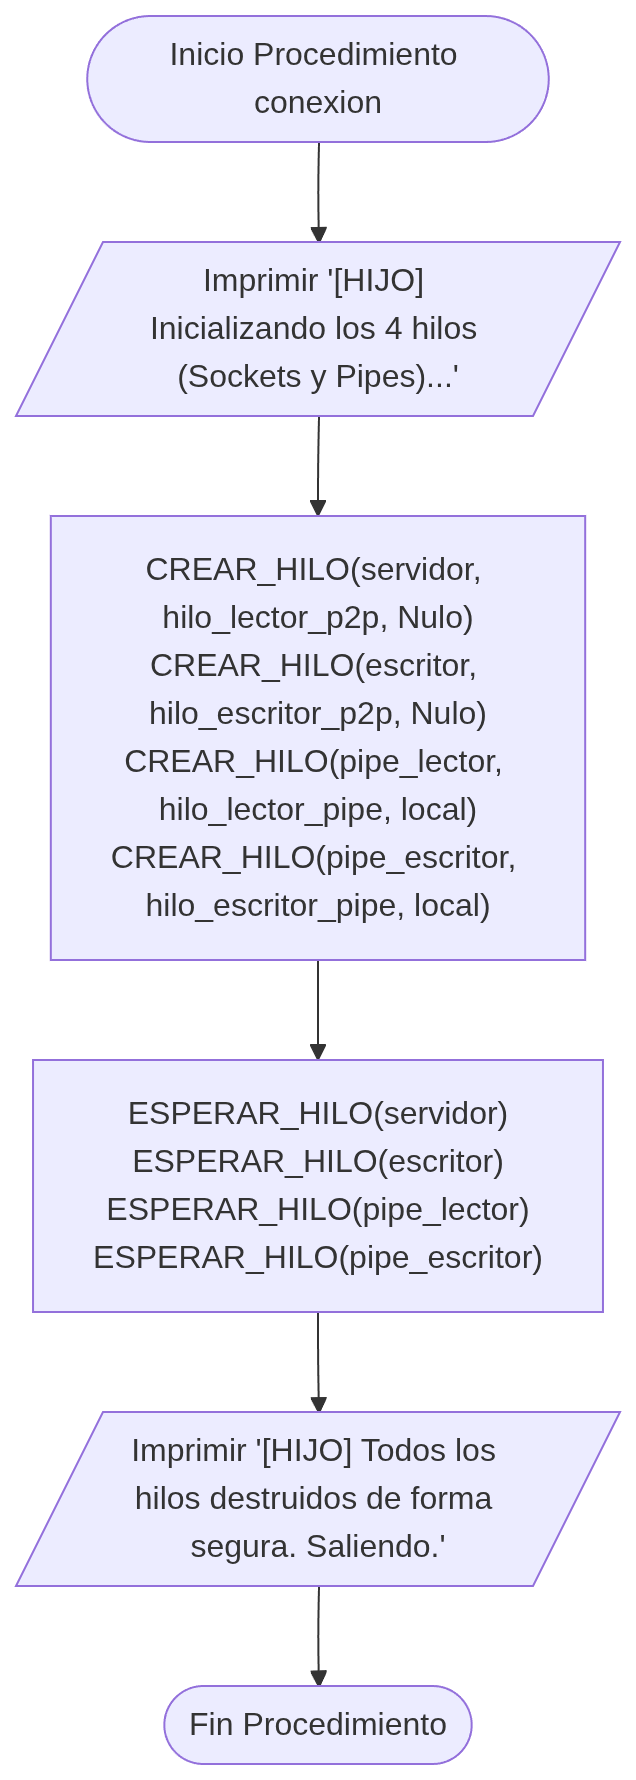
\includegraphics[width=0.25\textwidth]{Diagramas2/conexion.png} 
\end{figure}

% --- FUNCION 2 ---
\newpage
\paragraph{2.Función \texttt{hilo\_lector\_p2p()}} ~\\
\begin{figure}[H]
    \centering
    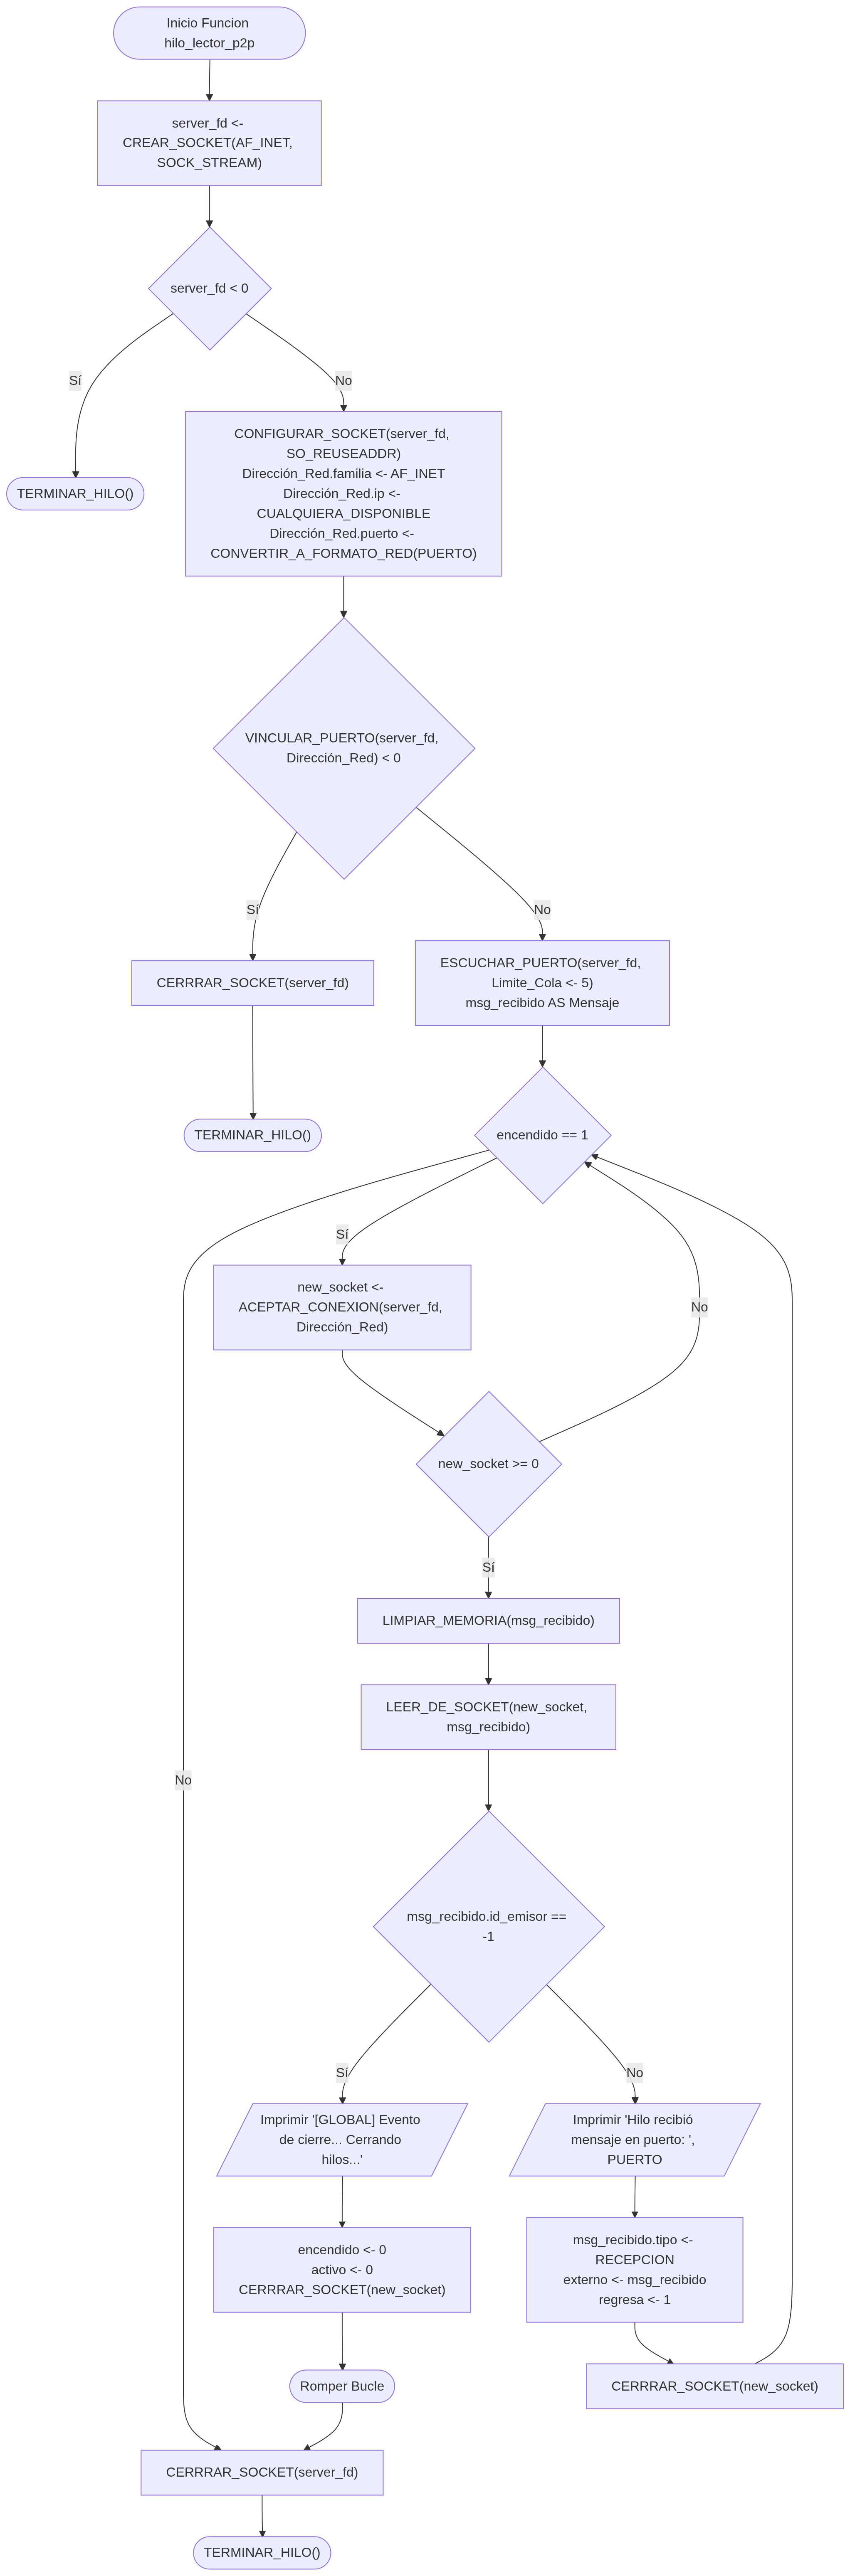
\includegraphics[width=0.35\textwidth]{Diagramas2/hilo_lector_p2p.png} 
\end{figure}

% --- FUNCION 3 ---
\newpage
\paragraph{3. Función \texttt{hilo\_escritor\_p2p()}} ~\\
\begin{figure}[H]
    \centering
    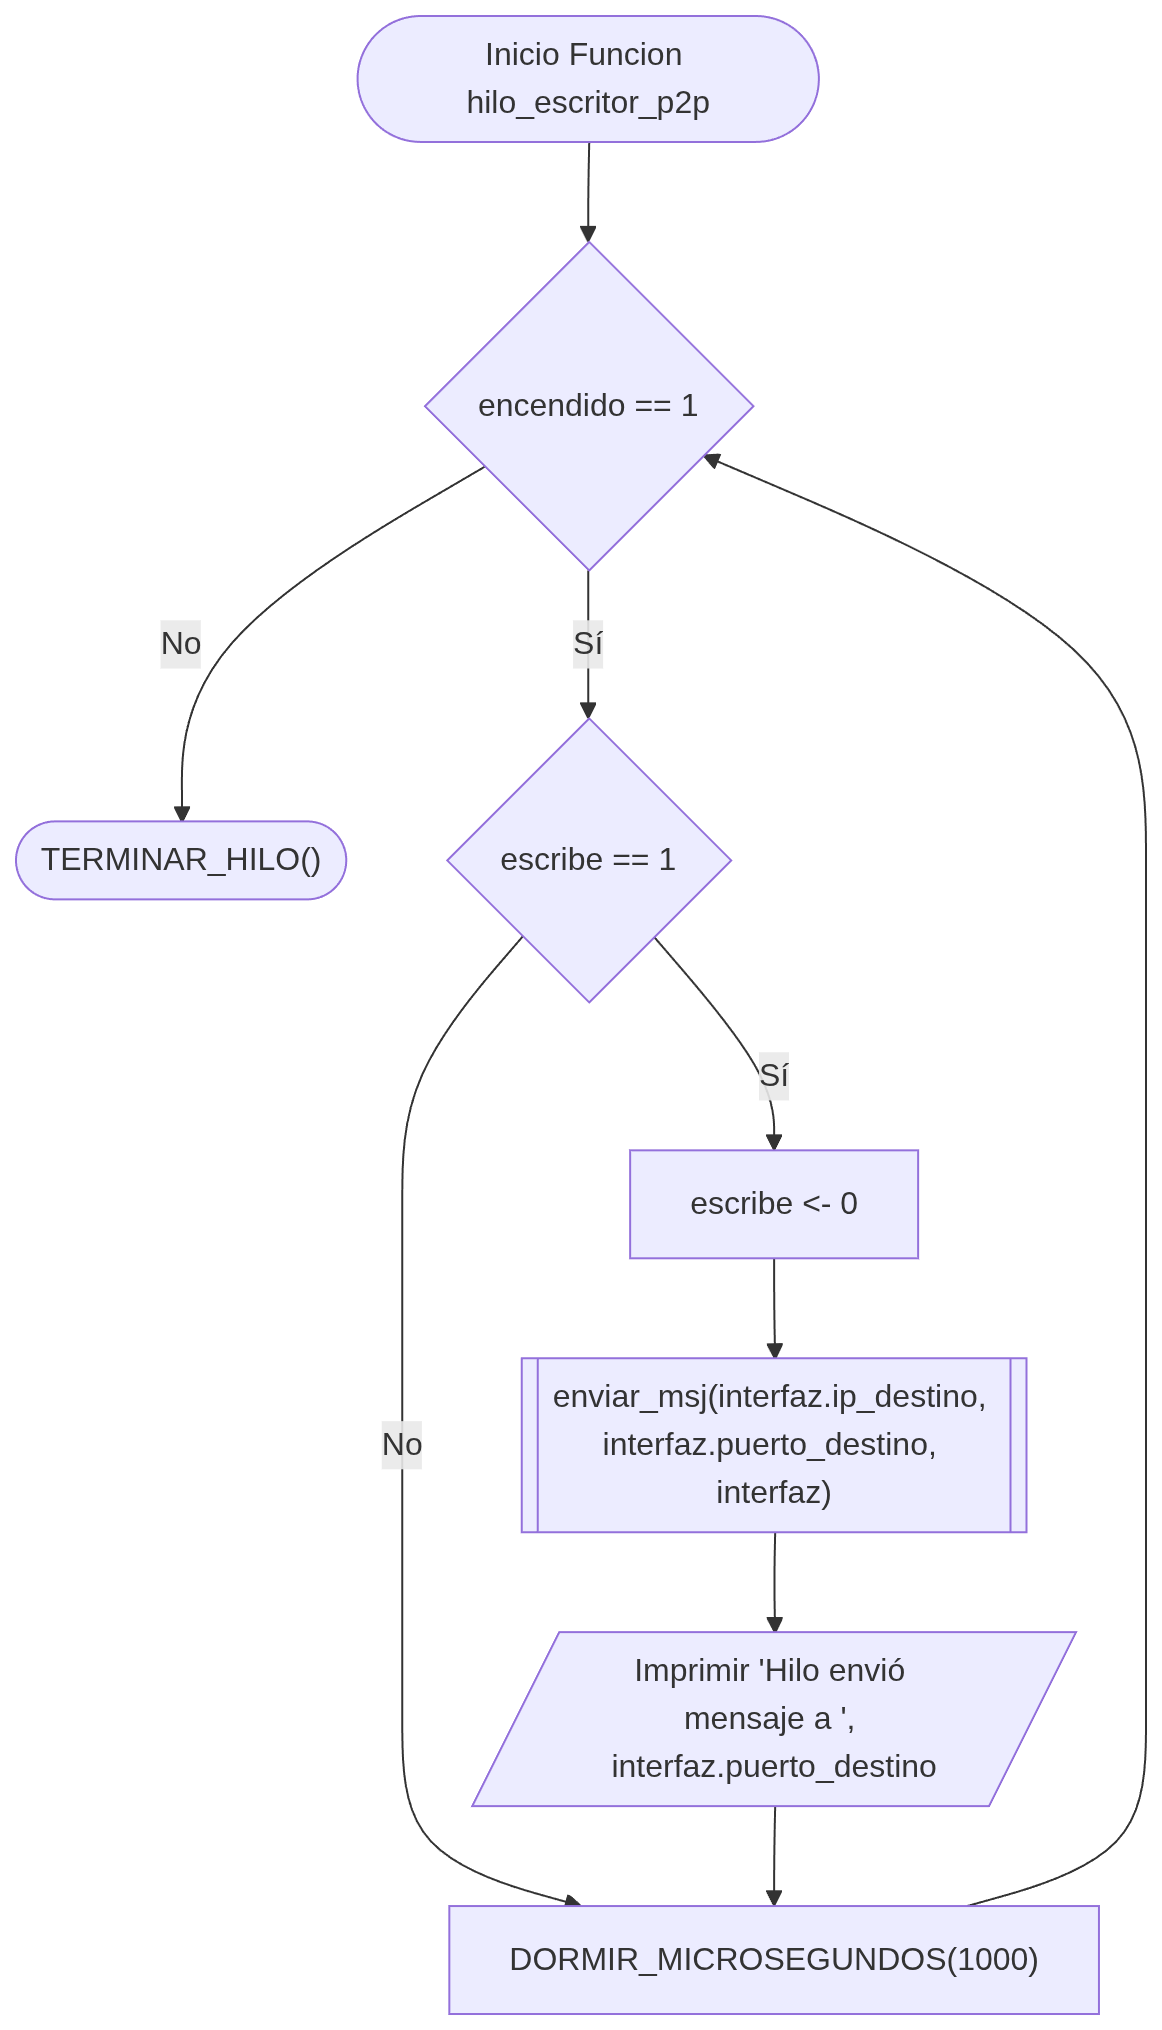
\includegraphics[width=0.4\textwidth]{Diagramas2/hilo_escritor_p2p.png} 
\end{figure}

% --- FUNCION 4 ---
\newpage
\paragraph{4. Función \texttt{hilo\_lector\_pipe()}} ~\\
\begin{figure}[H]
    \centering
    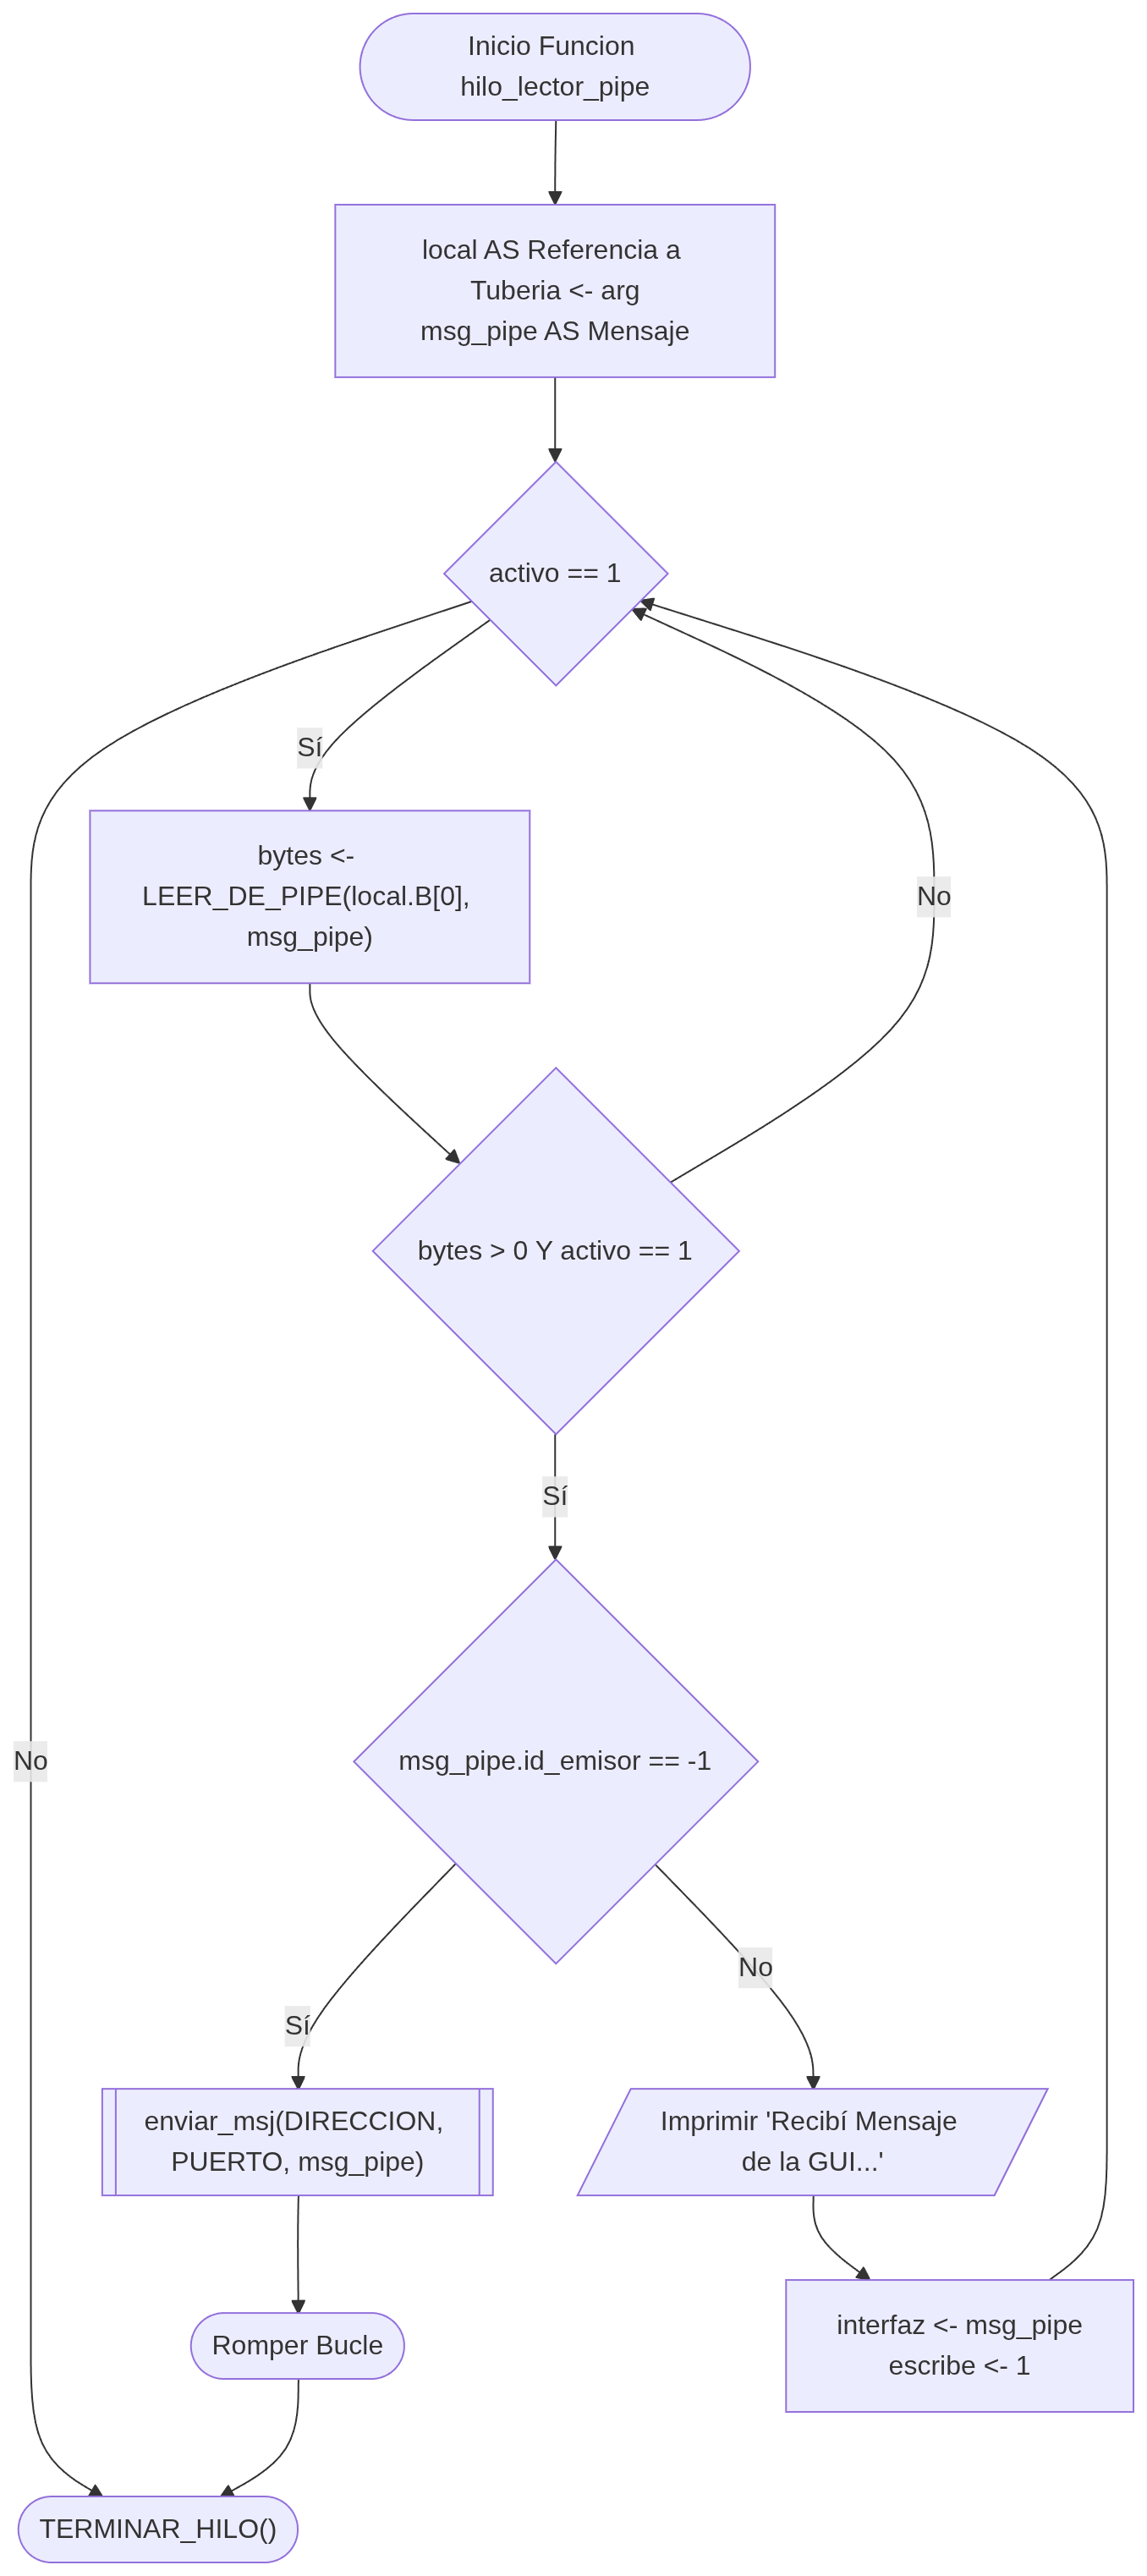
\includegraphics[width=0.4\textwidth]{Diagramas2/hilo_lector_pipe.png} 
\end{figure}

% --- FUNCION 5 ---
\newpage
\paragraph{5. Función \texttt{hilo\_escritor\_pipe()}} ~\\
\begin{figure}[H]
    \centering
    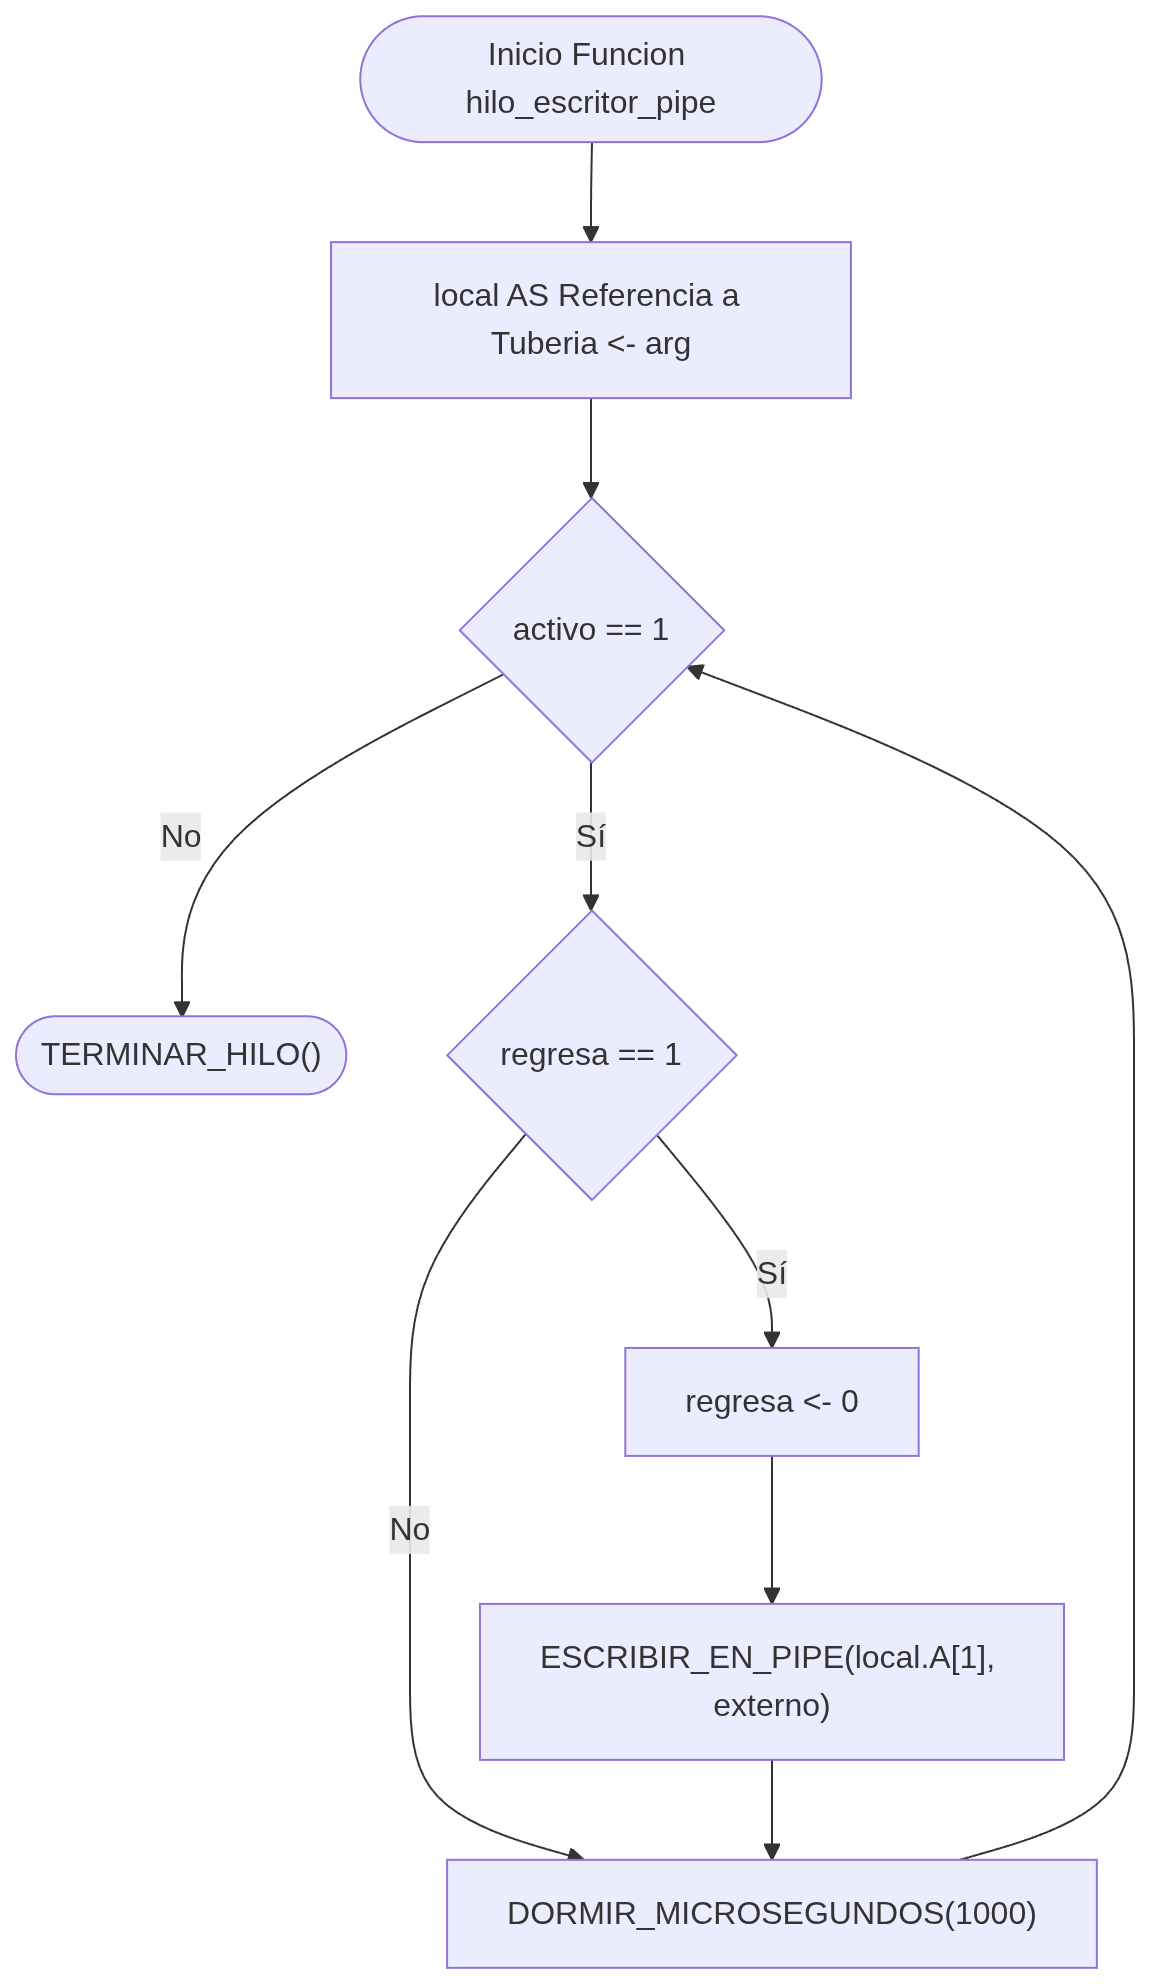
\includegraphics[width=0.4\textwidth]{Diagramas2/hilo_escritor_pipe.png} 
\end{figure}

% --- PROCEDIMIENTO 6 ---
\newpage
\paragraph{6. Procedimiento \texttt{enviar\_msj()}} ~\\
\begin{figure}[H]
    \centering
    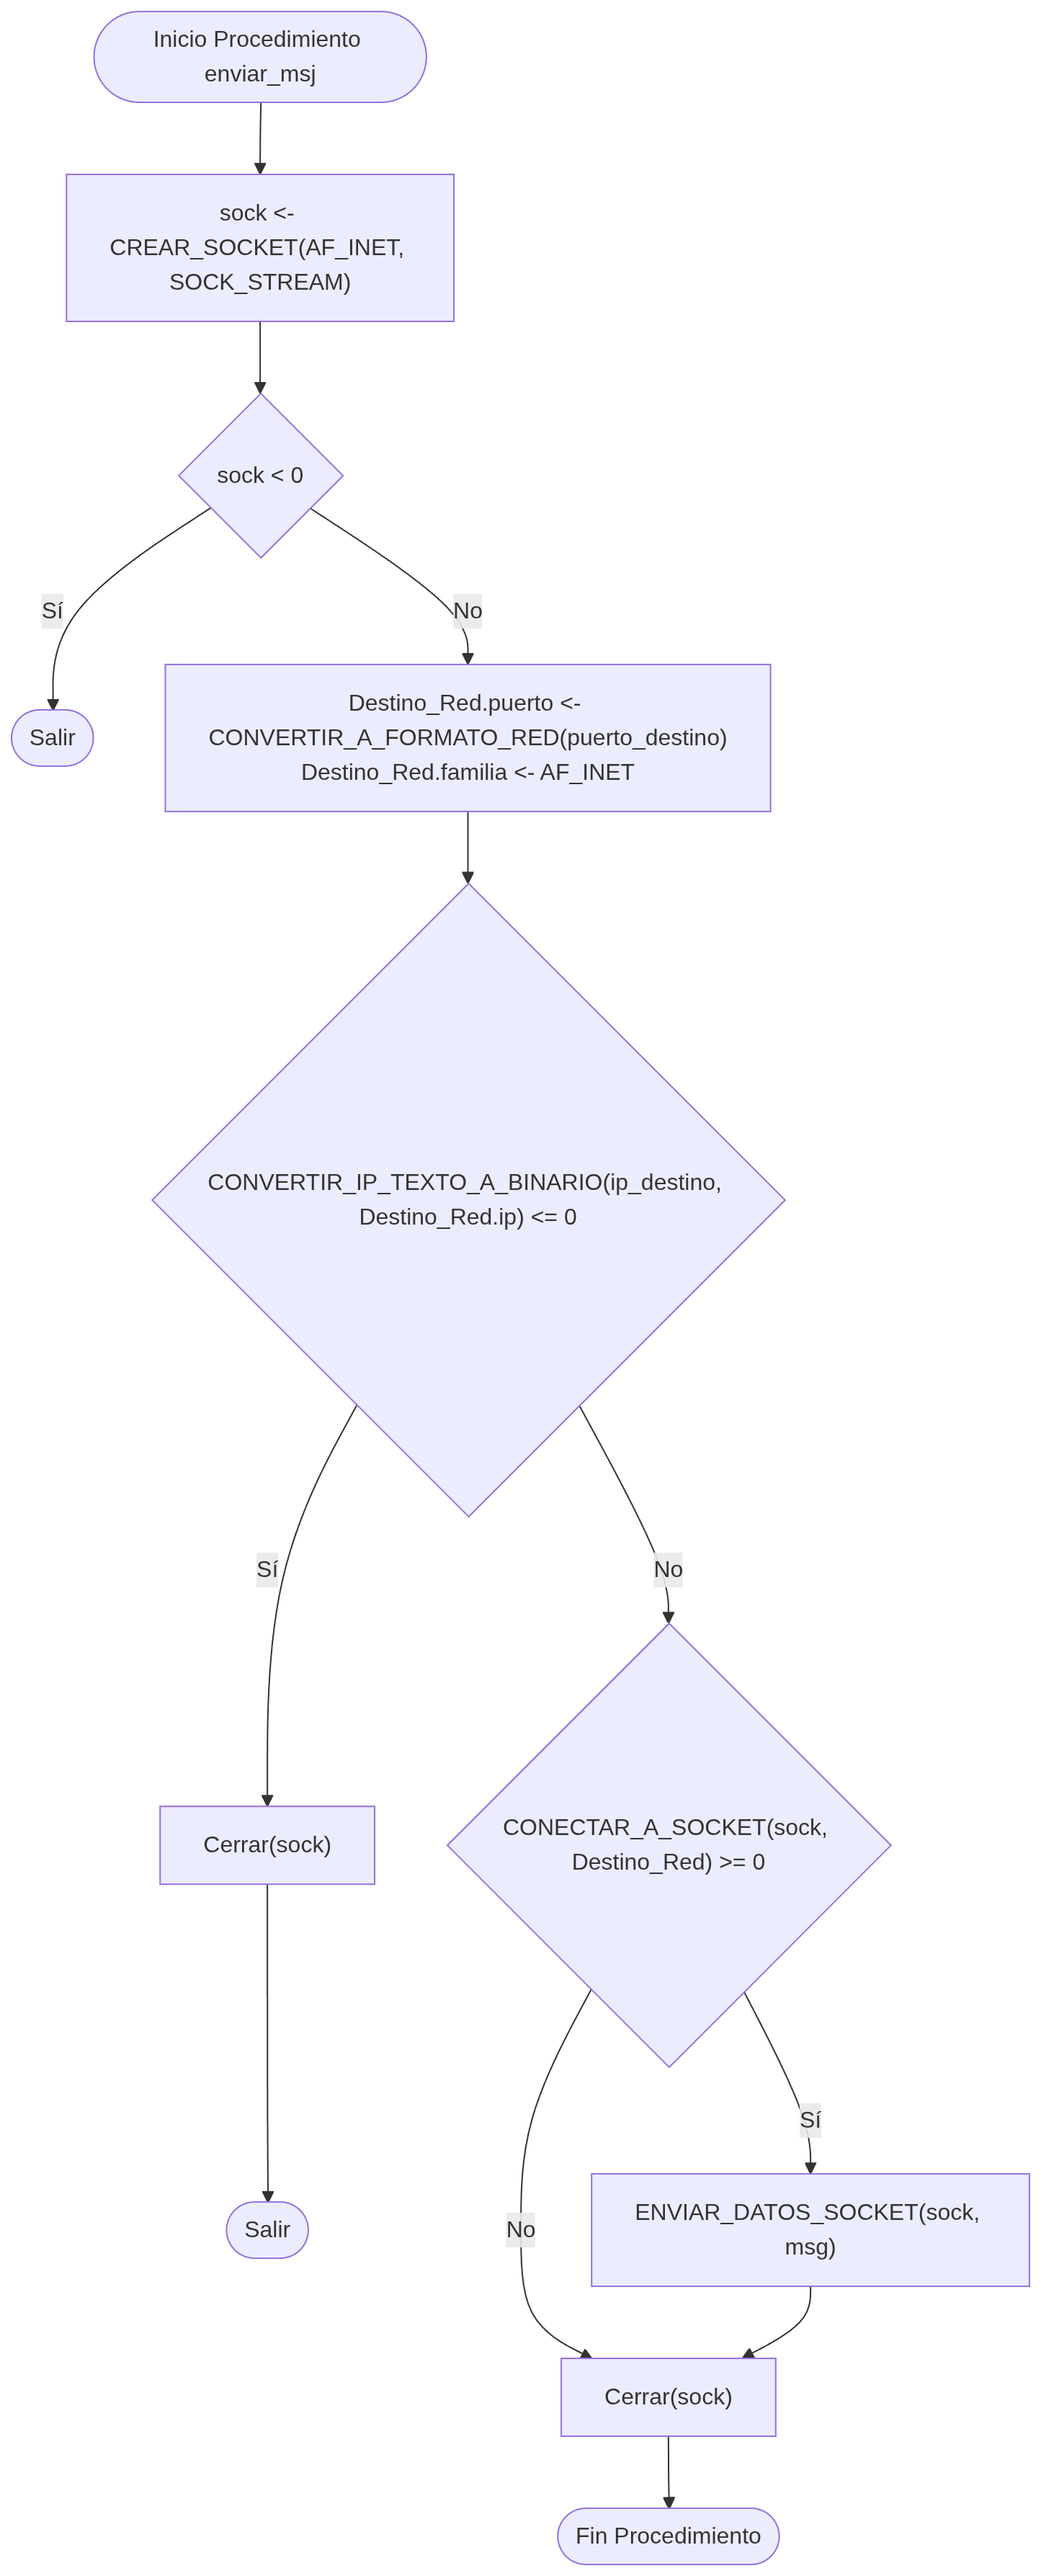
\includegraphics[width=0.4\textwidth]{Diagramas2/enviar_msj.png} 
\end{figure}

% --- FUNCION 7 Y 8 ---
\newpage
\paragraph{7. Función \texttt{get\_time\_ms()}} ~\\
\begin{figure}[H]
    \centering
    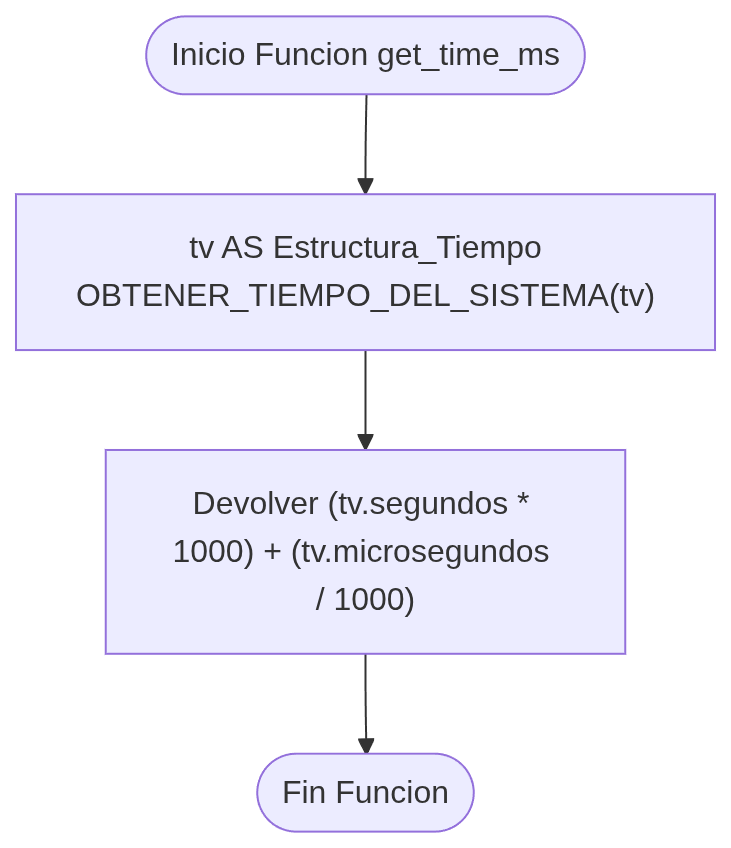
\includegraphics[width=0.25\textwidth]{Diagramas2/get_time_ms.png} 
\end{figure}

\paragraph{8. Procedimiento \texttt{formatear\_tiempo\_str()}} ~\\
\begin{figure}[H]
    \centering
    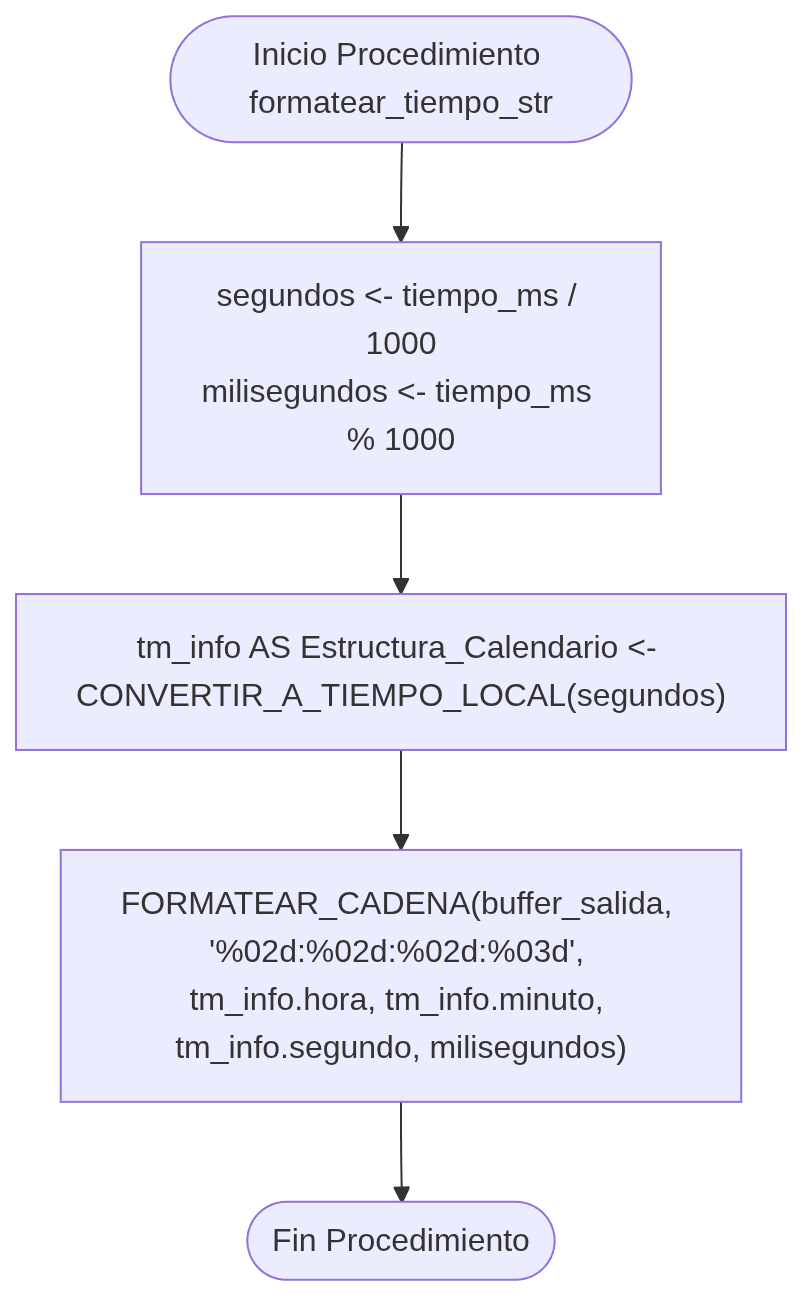
\includegraphics[width=0.25\textwidth]{Diagramas2/formatear_tiempo_str.png} 
\end{figure}
\subsection{\large Archivo de Interfaz Gráfica \texttt{(interfaz.c)}}
Este archivo, de la misma manera que la conexión, se manipula en un proceso independiente (\textit{frontend}) para que no se presenten problemas de congelamiento o bloqueos inesperados en la vista mientras la red opera. Utiliza la biblioteca \texttt{GTK+} para el renderizado visual y emplea \texttt{Pthreads} para mantener la comunicación asíncrona con el \textit{backend}.

A continuación, se detalla el funcionamiento de los bloques principales y subrutinas que conforman la lógica de la interfaz que se muestra al usuario principal:

\begin{itemize}
    \item \textbf{\texttt{interfaz\_grafica()}:} Es la subrutina maestra del \textit{frontend}. Inicializa el entorno gráfico de GTK, carga los recursos visuales CSS, y levanta los dos hilos (\texttt{gui\_lector} y \texttt{gui\_escritor}). Posteriormente, estructura jerárquicamente los contenedores (\texttt{GtkBox}, \texttt{GtkScrolledWindow}) y widgets (\texttt{GtkEntry}, \texttt{GtkButton}), cediendo finalmente el control al bucle principal de eventos (\texttt{gtk\_main()}).
    
    \item \textbf{Hilos IPC (\texttt{hilo\_lector\_gui} e \texttt{hilo\_escritor\_gui}):} Operan en segundo plano sin interferir con el renderizado de la ventana. El hilo lector extrae los datos entrantes del Pipe A de forma bloqueante y delega la actualización visual al hilo principal de GTK mediante \texttt{g\_idle\_add}. El hilo escritor evalúa activamente la bandera volátil \texttt{gui\_escribe} para transferir los mensajes del usuario hacia el \textit{backend} a través del Pipe B.
    
    \item \textbf{Gestión Visual (\texttt{añadir\_burbuja} y \texttt{mostrar\_mensaje\_recibido}):} Se encargan de instanciar las etiquetas (\texttt{GtkLabel}) para el texto del chat. Estas funciones evalúan la procedencia del mensaje (\texttt{es\_mio}) para anclar la alineación a la derecha (nodo local) o a la izquierda (nodo remoto). Utilizan la sintaxis \textit{Pango Markup} para dar formato a las estampas de tiempo y vinculan los ID del CSS para colorear las burbujas.
    
    \item \textbf{Persistencia (\texttt{cargar\_historial}, \texttt{guardar\_en\_historial}, \texttt{limpiar\_historial\_pulsado}):} Implementan un mecanismo local de almacenamiento en el archivo de texto \texttt{historial\_chat.txt}. Permiten serializar (usando el formato \texttt{Origen|Milisegundos|Texto}) y deserializar las cadenas para restaurar conversaciones de sesiones previas al abrir la aplicación, así como truncar el archivo para vaciar el registro.
    
    \item \textbf{Gestores de Eventos (\textit{Callbacks}):} 
    \begin{itemize}
        \item \textbf{\texttt{boton\_pulsado()}:} Captura el texto del cuadro de entrada al presionar Enter o dar clic en "Enviar", renderiza la burbuja local, lo almacena en disco y levanta la bandera para su envío IPC.
        \item \textbf{\texttt{ventana\_destruida()}:} Intercepta el cierre de la ventana por parte del usuario, empaquetando un mensaje especial (\texttt{id\_emisor = -1}) para forzar el apagado en cascada del \textit{backend} y cerrando el ciclo de GTK.
        \item \textbf{\texttt{scroll\_al\_final()}:} Ajusta dinámicamente el límite superior del \texttt{GtkAdjustment} para que la vista descienda automáticamente al insertar una nueva burbuja de diálogo.
    \end{itemize}
    
    \item \textbf{\texttt{cargar\_css()}:} Función integradora que instancia un \texttt{GtkCssProvider} para interpretar la hoja de estilos \texttt{v-boton.css}, inyectando los gradientes, bordes suavizados y colores distintivos del diseño tipo Messenger directamente al \texttt{GdkScreen} de la aplicación.
\end{itemize}

\begin{lstlisting}[style=estiloC, caption={Archivo del Front-End (conexion P2P)}]
#include <gtk/gtk.h>
#include <string.h>
#include <stdbool.h>
#include <unistd.h>
#include <pthread.h>
#include "header.h"

// Variables de control exclusivas para regular el ciclo de vida de los hilos de la GUI
volatile int gui_activo = 1;
// Bandera volatil para notificar que el usuario presiono enviar y hay datos listos para el pipe B
volatile int gui_escribe = 0;

// Buffers globales estructurados para la transferencia asincrona de informacion en la GUI
Mensaje msg_para_enviar;
Mensaje msg_recibido_pipe;

// Parametros de configuracion de red por defecto para el nodo remoto (amigo)
int puerto_amigo = 4001;        // El puerto en el que el otro extremo escucha conexiones
char dir_amigo[] = "127.0.0.1"; // Direccion IP del nodo remoto (mapeada localmente por defecto)
int puerto_actual = 4000;       // Puerto asignado a nuestra instancia para desplegarlo en la cabecera

// Componentes globales de GTK requeridos para la manipulacion de la vista desde multiples funciones
GtkWidget *caja_mensajes;
GtkAdjustment *adj_chat;
char buffer[TAM_MAX];

// Puntero de referencia global para interactuar con los descriptores de la tuberia principal IPC
Tuberia *gui_pipe_ref;

// Funcion de callback de baja prioridad para ajustar la barra de desplazamiento de forma automatica
static gboolean scroll_al_final(gpointer data)
{
    // Extraemos el limite superior maximo del area de scroll dinamicamente
    double max = gtk_adjustment_get_upper(adj_chat);
    // Obtenemos las dimensiones proporcionales de la pagina visible actual
    double page = gtk_adjustment_get_page_size(adj_chat);
    // Movemos el scroll al fondo absoluto restando el tamaño de la pagina visible al maximo alcanzado
    gtk_adjustment_set_value(adj_chat, max - page);
    // Retornamos FALSE para indicarle al planificador de GLib que destruya este evento tras ejecutarse una vez
    return FALSE;
}

// Subrutina encargada de construir los elementos visuales (widgets) para representar los mensajes del chat
static void añadir_burbuja(const char *texto, gboolean es_mio, long long tiempo_ms)
{
    // 1. Instanciamos una etiqueta de GTK para alojar la cadena del mensaje enviado o recibido
    GtkWidget *burbuja = gtk_label_new(texto);
    // Habilitamos el ajuste de linea automatico si el texto supera las dimensiones horizontales maximas
    gtk_label_set_line_wrap(GTK_LABEL(burbuja), TRUE);
    // Configuramos que la ruptura de linea se haga por palabras y caracteres de forma limpia
    gtk_label_set_line_wrap_mode(GTK_LABEL(burbuja), PANGO_WRAP_WORD_CHAR);
    // Establecemos una restriccion de diseño fijando el ancho maximo en 35 caracteres por fila
    gtk_label_set_max_width_chars(GTK_LABEL(burbuja), 35);

    // 2. Declaramos y formateamos la cadena que mostrara la estampa de tiempo
    char str_tiempo[32];
    char markup_tiempo[128];
    formatear_tiempo_str(tiempo_ms, str_tiempo);

    // Formateamos usando sintaxis Pango Markup para reducir la fuente (font='8') y conservar un color oscuro
    sprintf(markup_tiempo, "<span font='8' foreground='#000000'>%s</span>", str_tiempo);
    GtkWidget *label_tiempo = gtk_label_new(NULL);
    // Inyectamos el formato enriquecido en la etiqueta correspondiente
    gtk_label_set_markup(GTK_LABEL(label_tiempo), markup_tiempo);

    // Alineamos verticalmente la etiqueta del tiempo al centro para mantener simetria visual
    gtk_widget_set_valign(label_tiempo, GTK_ALIGN_CENTER);

    // 3. Creamos un contenedor horizontal (HBox) para estructurar la linea del mensaje actual
    GtkWidget *alineacion = gtk_box_new(GTK_ORIENTATION_HORIZONTAL, 0);
    // Asignamos margenes externos a la burbuja para que no quede pegada a las paredes ni a otras burbujas
    gtk_widget_set_margin_start(burbuja, 15);
    gtk_widget_set_margin_end(burbuja, 15);
    gtk_widget_set_margin_top(burbuja, 5);
    gtk_widget_set_margin_bottom(burbuja, 5);

    // Condicional para ramificar el diseño estilo Messenger dependiendo de la procedencia del mensaje
    if (es_mio)
    {
        // Si es propio, alineamos todo el contenedor a la extrema derecha
        gtk_widget_set_halign(alineacion, GTK_ALIGN_END);
        // Le asignamos el ID CSS "mi-mensaje" definido en v-boton.css (azul con bordes suavizados)
        gtk_widget_set_name(burbuja, "mi-mensaje");

        // Estructuramos la distribucion: primero la estampa de tiempo, luego el texto a la derecha
        gtk_box_pack_start(GTK_BOX(alineacion), label_tiempo, FALSE, FALSE, 0);
        gtk_box_pack_start(GTK_BOX(alineacion), burbuja, FALSE, FALSE, 0);
    }
    else
    {
        // Si proviene de la red, alineamos el contenedor a la extrema izquierda
        gtk_widget_set_halign(alineacion, GTK_ALIGN_START);
        // Le asignamos el ID CSS "su-mensaje" definido en v-boton.css (rojo/guinda)
        gtk_widget_set_name(burbuja, "su-mensaje");

        // Estructuramos la distribucion: primero el texto, luego la estampa de tiempo a la derecha
        gtk_box_pack_start(GTK_BOX(alineacion), burbuja, FALSE, FALSE, 0);
        gtk_box_pack_start(GTK_BOX(alineacion), label_tiempo, FALSE, FALSE, 0);
    }

    // Insertamos la fila estructurada dentro de la caja contenedora vertical del chat
    gtk_container_add(GTK_CONTAINER(caja_mensajes), alineacion);
    // Forzamos el renderizado inmediato del nuevo componente y sus widgets secundarios
    gtk_widget_show_all(alineacion);

    // Agregamos la rutina de autoscroll al bucle principal de eventos para ejecutarse en el proximo ciclo de ocio
    g_idle_add(scroll_al_final, NULL);
}

// Funcion para persistir de forma local e incremental la bitacora de conversacion
void guardar_en_historial(const char *texto, gboolean es_mio, long long tiempo_ms) {
    // Abrimos el archivo en modo "a" (append) para añadir nuevas lineas al final del documento sin sobreescribir
    FILE *archivo = fopen("historial_chat.txt", "a"); 
    if (archivo != NULL) {
        // Almacenamos los datos serializados bajo el delimitador de tuberia: [Origen]|[Milisegundos]|[Texto]
        fprintf(archivo, "%d|%lld|%s\n", es_mio ? 1 : 0, tiempo_ms, texto);
        // Cerramos el flujo del archivo para asegurar la descarga fisica de datos en el disco
        fclose(archivo);
    }
}

// Callback intermedio invocado de forma segura por el hilo principal de GTK para procesar buffers remotos
static gboolean mostrar_mensaje_recibido(gpointer data)
{
    // Construimos graficamente la burbuja correspondiente a la izquierda utilizando los datos del pipe
    añadir_burbuja(msg_recibido_pipe.texto, FALSE, msg_recibido_pipe.tiempo);
    // Respaldamos de forma permanente el mensaje remoto en el archivo de texto local
    guardar_en_historial(msg_recibido_pipe.texto, FALSE, msg_recibido_pipe.tiempo);
    // Retornamos FALSE para liberar el callback del despachador principal de eventos
    return FALSE;
}

// Subrutina invocada al arranque para reconstruir la sesion anterior a partir del archivo de historial
void cargar_historial() {
    // Abrimos el archivo en modo lectura estricta
    FILE *archivo = fopen("historial_chat.txt", "r"); 
    // Si el archivo no existe en el directorio, abortamos la operacion limpiamente sin lanzar excepciones
    if (archivo == NULL) return; 

    char linea[TAM_MAX + 100]; 
    // Leemos secuencialmente linea por linea hasta llegar al final del archivo de texto
    while (fgets(linea, sizeof(linea), archivo) != NULL) {
        // Removemos de forma segura el caracter de salto de linea '\n' remanente de fgets
        linea[strcspn(linea, "\n")] = 0;

        int es_mio = 0;
        long long tiempo_ms = 0;
        char texto[TAM_MAX] = {0};

        // Encontramos el primer token de division '|' correspondiente al bit de procedencia
        char *ptr1 = strchr(linea, '|');
        if (ptr1) {
            *ptr1 = '\0'; // Dividimos la cadena temporalmente introduciendo un terminador nulo
            es_mio = atoi(linea); // Convertimos el fragmento ASCII a entero ordinario (0 o 1)
            
            // Encontramos el segundo token correspondiente al timestamp en milisegundos
            char *ptr2 = strchr(ptr1 + 1, '|');
            if (ptr2) {
                *ptr2 = '\0'; // Dividimos el fragmento final
                tiempo_ms = atoll(ptr1 + 1); // Convertimos la cadena de texto a entero largo de 64 bits (long long)
                strcpy(texto, ptr2 + 1);     // Extraemos el texto integro restante del mensaje
                
                // Pintamos la burbuja retrospectivamente preservando si era local o remota
                añadir_burbuja(texto, es_mio == 1 ? TRUE : FALSE, tiempo_ms);
            }
        }
    }
    // Cerramos el descriptor de lectura una vez concluida la carga inicial
    fclose(archivo);
}

// Callback de evento activado al pulsar el boton "Limpiar"
static void limpiar_historial_pulsado(GtkWidget *widget, gpointer data)
{
    // 1. Truncamos y vaciamos por completo el archivo de historial abriendolo en modo escritura "w"
    FILE *archivo = fopen("historial_chat.txt", "w");
    if (archivo != NULL) {
        fclose(archivo); // Al cerrarse de inmediato, el archivo queda vacio con 0 bytes
    }

    // 2. Iteramos sobre cada widget hijo contenido en la caja de mensajes y lo destruimos fisicamente
    gtk_container_foreach(GTK_CONTAINER(caja_mensajes), (GtkCallback)gtk_widget_destroy, NULL);
    
    // Desplegamos bitacora de control en consola
    printf("[GUI] Historial limpiado.\n");
}

// Callback invocado cuando el usuario hace clic en el boton Enviar o presiona Enter en la entrada de texto
static void boton_pulsado(GtkWidget *widget, gpointer data)
{
    GtkEntry *entry = GTK_ENTRY(data);
    // Recuperamos el buffer de texto plano de la caja de entrada de GTK
    const char *texto = gtk_entry_get_text(entry);

    // Proteccion elemental: solo procesamos la entrada si contiene caracteres validos
    if (strlen(texto) > 0)
    {
        // Registramos inmediatamente el tiempo del sistema en milisegundos para estampar la operacion
        long long mi_tiempo = get_time_ms();
        // Agregamos la representacion grafica del mensaje propio apuntando a la derecha
        añadir_burbuja(texto, TRUE, mi_tiempo);

        // Almacenamos localmente el mensaje en la bitacora persistente
        guardar_en_historial(texto, TRUE, mi_tiempo);

        // Empaquetamos y serializamos los datos crudos en la estructura Mensaje para su transmision IPC
        msg_para_enviar.id_emisor = getpid(); // Identificador unico del proceso emisor (Frontend)
        msg_para_enviar.tipo = ENVIO;         // Clasificamos la operacion como un mensaje de salida
        strncpy(msg_para_enviar.texto, texto, sizeof(msg_para_enviar.texto) - 1);
        strncpy(msg_para_enviar.ip_destino, dir_amigo, sizeof(msg_para_enviar.ip_destino) - 1);
        msg_para_enviar.puerto_destino = puerto_amigo;
        msg_para_enviar.tiempo = mi_tiempo;   // Guardamos el timestamp sincronizado para la transmision

        // Alzamos la bandera volatil para desbloquear la ejecucion del hilo escritor de la interfaz
        gui_escribe = 1;

        // Vaciamos la caja de texto para dejarla disponible para el proximo mensaje
        gtk_entry_set_text(entry, "");
    }
}

// Manejador del evento de destruccion de la ventana (Cierre de la aplicacion)
static void ventana_destruida(GtkWidget *widget, gpointer data)
{
    printf("[GUI] Cerrando ventana. Enviando señal de apagado...\n");

    // Preparamos un mensaje de control especial inyectando -1 en el emisor
    msg_para_enviar.id_emisor = -1;
    msg_para_enviar.tipo = SALIDA;
    strncpy(msg_para_enviar.texto, "Cierre de interfaz.", sizeof(msg_para_enviar.texto) - 1);
    
    // Forzamos una escritura bloqueante sincrona en el pipe B hacia el backend para ordenar su apagado masivo
    write(gui_pipe_ref->B[1], &msg_para_enviar, sizeof(Mensaje));
    
    // Bajamos las banderas globales de control para romper los ciclos infinitos de los hilos remanentes
    gui_escribe = 0; 
    gui_activo = 0; 
    
    // Rompemos el bucle principal de GTK para devolver la ejecucion al hilo principal
    gtk_main_quit();
}

// Cargador e interprete del archivo de diseño en cascada CSS para GTK
void cargar_css(void)
{
    // Instanciamos un proveedor de estilos CSS para GTK
    GtkCssProvider *provider = gtk_css_provider_new();
    // Recuperamos la pantalla por defecto asignada al entorno grafico actual
    GdkDisplay *display = gdk_display_get_default();
    GdkScreen *screen = gdk_display_get_default_screen(display);
    
    // Leemos e interpretamos los selectores declarados en "v-boton.css"
    gtk_css_provider_load_from_path(provider, "v-boton.css", NULL);
    // Aplicamos los estilos de forma global a la pantalla con prioridad de aplicacion para sobreescribir temas nativos
    gtk_css_provider_add_provider_for_screen(screen, GTK_STYLE_PROVIDER(provider), GTK_STYLE_PROVIDER_PRIORITY_APPLICATION);
    // Decrementamos el contador de referencias del proveedor para liberar memoria limpia
    g_object_unref(provider);
}

// === HILO 1 DE LA GUI: Lector dedicado en segundo plano para el Pipe A ===
void *hilo_lector_gui(void *arg)
{
    Tuberia *local = (Tuberia *)arg;
    printf("[GUI-HILO-LECTOR] Hilo de lectura de pipe iniciado...\n");

    // Se ejecutara de fondo mientras dure la sesion grafica sin interrumpir los hilos de render
    while (gui_activo)
    {
        Mensaje temporal;
        // Operacion bloqueante a nivel de Kernel: espera paquetes provenientes del backend en el pipe A[0]
        int bytes = read(local->A[0], &temporal, sizeof(Mensaje));

        // Validamos que se hayan extraido bytes coherentes y la interfaz siga en estado activo
        if (bytes > 0 && gui_activo)
        {
            // Si el mensaje entrante fue catalogado por el backend como una RECEPCION de red
            if (temporal.tipo == RECEPCION)
            {
                printf("Recibi mensaje de la conexion...\n");
                // Mapeamos los datos de forma segura en la estructura global dedicada a la GUI
                memcpy(&msg_recibido_pipe, &temporal, sizeof(Mensaje));
                // Delegamos de forma asincrona e indolora la insercion grafica en el hilo principal de GTK
                g_idle_add(mostrar_mensaje_recibido, NULL);
            }
        }
        else
        {
            // Si el descriptor es cerrado o da error, rompemos el ciclo de ejecucion de forma inmediata
            break;
        }
    }
    printf("[GUI-HILO-LECTOR] Saliendo del hilo lector de la interfaz.\n");
    // Terminamos de forma limpia e independiente la existencia de este hilo
    pthread_exit(NULL);
}

// === HILO 2 DE LA GUI: Escritor dedicado en segundo plano para canalizar en el Pipe B ===
void *hilo_escritor_gui(void *arg)
{
    Tuberia *local = (Tuberia *)arg;
    printf("[GUI-HILO-ESCRITOR] Hilo de escritura de pipe iniciado...\n");

    while (gui_activo)
    {
        // Evaluamos de forma constante mediante sondeo (polling) el estado de la bandera de salida
        if (gui_escribe == 1)
        {
            // Despachamos la estructura serializada por el pipe B para que el modulo de red lo procese
            write(local->B[1], &msg_para_enviar, sizeof(Mensaje));
            // Apagamos la señal inmediatamente para evitar reenvios duplicados
            gui_escribe = 0; 
        }
        // Dormimos el hilo durante 1 milisegundo para evitar que el bucle vacio consuma el 100% de un nucleo del CPU
        usleep(1000); 
    }
    printf("[GUI-HILO-ESCRITOR] Saliendo del hilo escritor de la interfaz.\n");
    pthread_exit(NULL);
}

// Inicializador maestro de la interfaz grafica de usuario
void interfaz_grafica(int argc, char *argv[], Tuberia *padre)
{
    // Descriptores internos para almacenar la configuracion geometrica y jerarquica de los componentes de GTK
    GtkWidget *window, *box, *entry, *scrolled_window, *hbox, *button, *header_box, *info_contacto;
    pthread_t gui_lector, gui_escritor;

    // Resguardamos localmente la direccion de memoria del canal de pipes cruzados
    gui_pipe_ref = padre;

    // Inicializamos el entorno basico de GTK abstrayendo los argumentos de linea de comandos
    gtk_init(&argc, &argv);
    // Inyectamos las hojas de estilo personalizadas estilo Messenger retro-futurista
    cargar_css();

    // --- CONCURRENCIA: LEVANTAR LOS DOS HILOS INDEPENDIENTES DE LA GUI ---
    pthread_create(&gui_lector, NULL, hilo_lector_gui, (void *)gui_pipe_ref);
    pthread_create(&gui_escritor, NULL, hilo_escritor_gui, (void *)gui_pipe_ref);

    // Construimos la ventana principal y definimos sus atributos generales
    window = gtk_window_new(GTK_WINDOW_TOPLEVEL);
    gtk_window_set_title(GTK_WINDOW(window), "MSN P2P - INTERFAZ");
    gtk_window_set_default_size(GTK_WINDOW(window), 450, 650);

    // Vinculamos la señal de destruccion fisica de la ventana al callback de control ventana_destruida
    g_signal_connect(window, "destroy", G_CALLBACK(ventana_destruida), NULL);

    // Contenedor base vertical que apilara la cabecera, la caja de texto y la seccion de entrada
    box = gtk_box_new(GTK_ORIENTATION_VERTICAL, 0);
    gtk_container_add(GTK_CONTAINER(window), box);

    // --- DISEÑO DE LA CABECERA (Header estilo MSN) ---
    header_box = gtk_box_new(GTK_ORIENTATION_HORIZONTAL, 10);
    gtk_widget_set_name(header_box, "header-messenger");
    gtk_box_pack_start(GTK_BOX(box), header_box, FALSE, FALSE, 0);
    info_contacto = gtk_label_new(NULL);

    // Redactamos el banner informativo inyectando etiquetas con formato enriquecido mediante snprintf
    snprintf(buffer, sizeof(buffer),
             "<span font='11' weight='bold' foreground='#003399'>MESSENGER P2P</span>\n"
             "<span font='9' foreground='#666'>Escucha: %d - Conectado</span>",
             puerto_actual);

    gtk_label_set_markup(GTK_LABEL(info_contacto), buffer);
    gtk_box_pack_start(GTK_BOX(header_box), info_contacto, FALSE, FALSE, 15);

    // --- COMPONENTE COMPLEMENTARIO: BOTON DE LIMPIEZA DE BITACORA ---
    GtkWidget *btn_limpiar = gtk_button_new_with_label("Limpiar");
    g_signal_connect(btn_limpiar, "clicked", G_CALLBACK(limpiar_historial_pulsado), NULL);
    // Empaquetamos el boton al final (pack_end) para arrastrarlo al extremo derecho de la cabecera
    gtk_box_pack_end(GTK_BOX(header_box), btn_limpiar, FALSE, FALSE, 15);

    // --- COMPONENTE DE DESPLAZAMIENTO (Scrolled Window) ---
    scrolled_window = gtk_scrolled_window_new(NULL, NULL);
    gtk_box_pack_start(GTK_BOX(box), scrolled_window, TRUE, TRUE, 0);
    // Extraemos la configuracion geometrica del ajuste vertical para controlar la posicion de la barra
    adj_chat = gtk_scrolled_window_get_vadjustment(GTK_SCROLLED_WINDOW(scrolled_window));

    // Instanciamos el contenedor interno vertical donde se iran apilando dinamicamente las lineas del chat
    caja_mensajes = gtk_box_new(GTK_ORIENTATION_VERTICAL, 0);
    gtk_widget_set_valign(caja_mensajes, GTK_ALIGN_END); // Anclamos el crecimiento hacia abajo
    gtk_container_add(GTK_CONTAINER(scrolled_window), caja_mensajes);

    // --- AREA INFERIOR DE CAPTURA (HBox de entrada y transmision) ---
    hbox = gtk_box_new(GTK_ORIENTATION_HORIZONTAL, 5);
    gtk_widget_set_margin_start(hbox, 10);
    gtk_widget_set_margin_end(hbox, 10);
    gtk_widget_set_margin_top(hbox, 10);
    gtk_widget_set_margin_bottom(hbox, 10);
    gtk_box_pack_start(GTK_BOX(box), hbox, FALSE, FALSE, 0);

    // Instanciamos el cuadro de entrada de texto plano (GtkEntry)
    entry = gtk_entry_new();
    gtk_entry_set_placeholder_text(GTK_ENTRY(entry), "Escribe un mensaje...");
    
    // Conectamos el evento "activate" (presionar Enter dentro del cuadro) al callback boton_pulsado
    g_signal_connect(entry, "activate", G_CALLBACK(boton_pulsado), entry);
    gtk_box_pack_start(GTK_BOX(hbox), entry, TRUE, TRUE, 0);

    // Instanciamos el boton fisico de Enviar
    button = gtk_button_new_with_label("Enviar");
    // Conectamos el click del raton al mismo callback compartiendo el puntero de la caja de texto
    g_signal_connect(button, "clicked", G_CALLBACK(boton_pulsado), entry);
    gtk_box_pack_start(GTK_BOX(hbox), button, FALSE, FALSE, 0);

    // Reconstruimos la conversacion anterior leyendo de disco antes de levantar la interfaz visible
    cargar_historial();

    // Mostramos la ventana y ordenamos la cascada jerarquica de widgets internos
    gtk_widget_show_all(window);
    
    // Bloqueamos el hilo principal cediendo el control total al despachador de eventos de GTK (Bucle principal)
    gtk_main();

    // Sincronizacion final: Al romperse el bucle, esperamos la terminacion e incorporacion de los hilos asincronos
    pthread_join(gui_lector, NULL);
    pthread_join(gui_escritor, NULL);
}
\end{lstlisting}
\input{pseudocodigo3.tex}
\subsubsection{\large Diagrama de flujo \texttt{(interfaz.c)}}

% --- PROCEDIMIENTO 1 ---
\newpage
\paragraph{1. Procedimiento \texttt{interfaz\_grafica()}} ~\\
\begin{figure}[H]
    \centering
    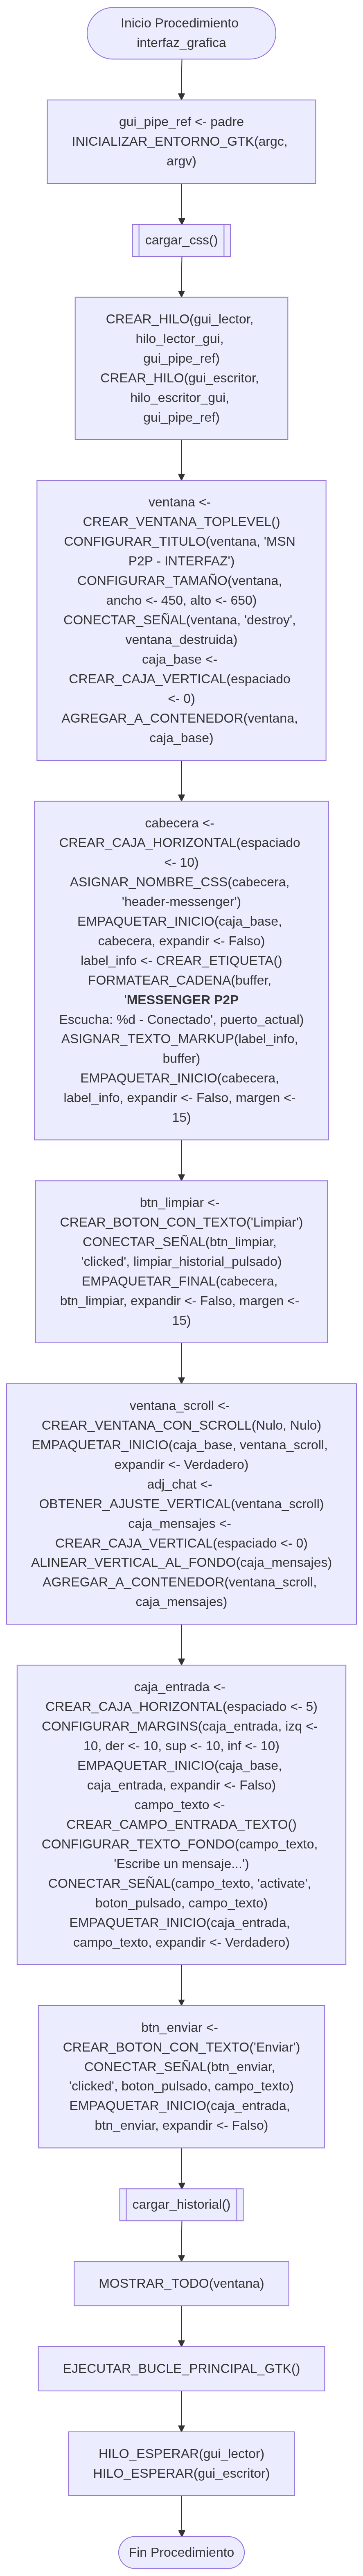
\includegraphics[width=0.15\textwidth]{Diagramas3/interfaz_grafica.png} 
\end{figure}

% --- FUNCION 2 ---
\newpage
\paragraph{2. Función \texttt{hilo\_lector\_gui()}} ~\\
\begin{figure}[H]
    \centering
    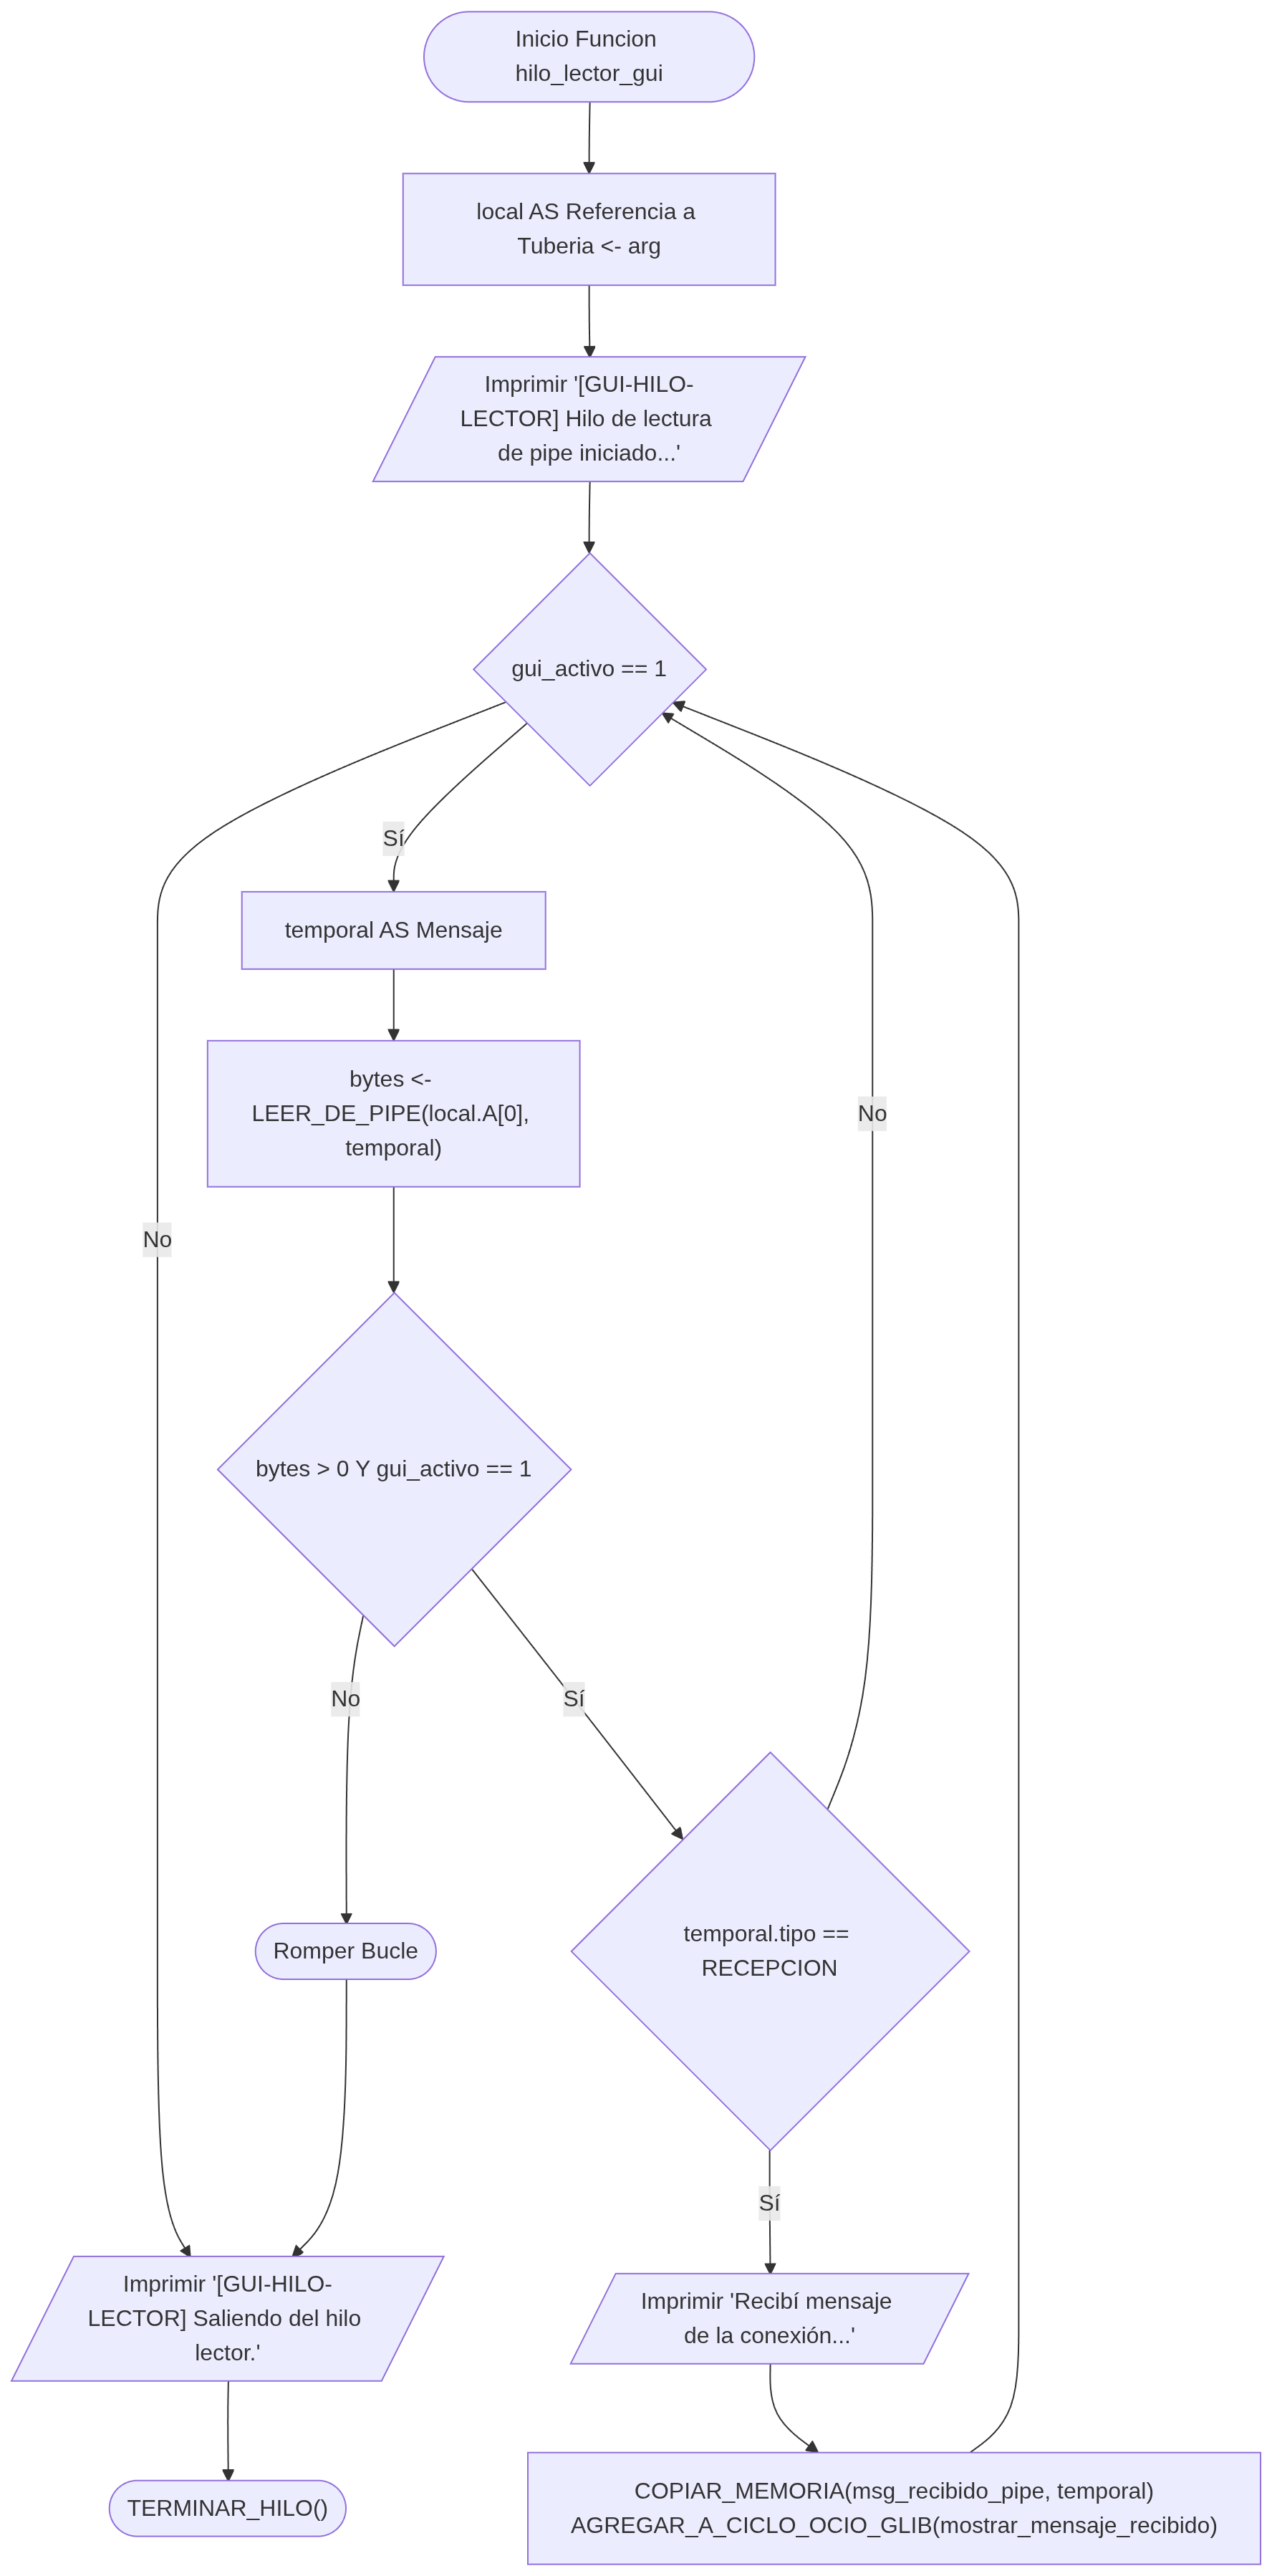
\includegraphics[width=0.5\textwidth]{Diagramas3/hilo_lector_gui.png} 
\end{figure}

% --- FUNCION 3 ---
\newpage
\paragraph{3. Función \texttt{hilo\_escritor\_gui()}} ~\\
\begin{figure}[H]
    \centering
    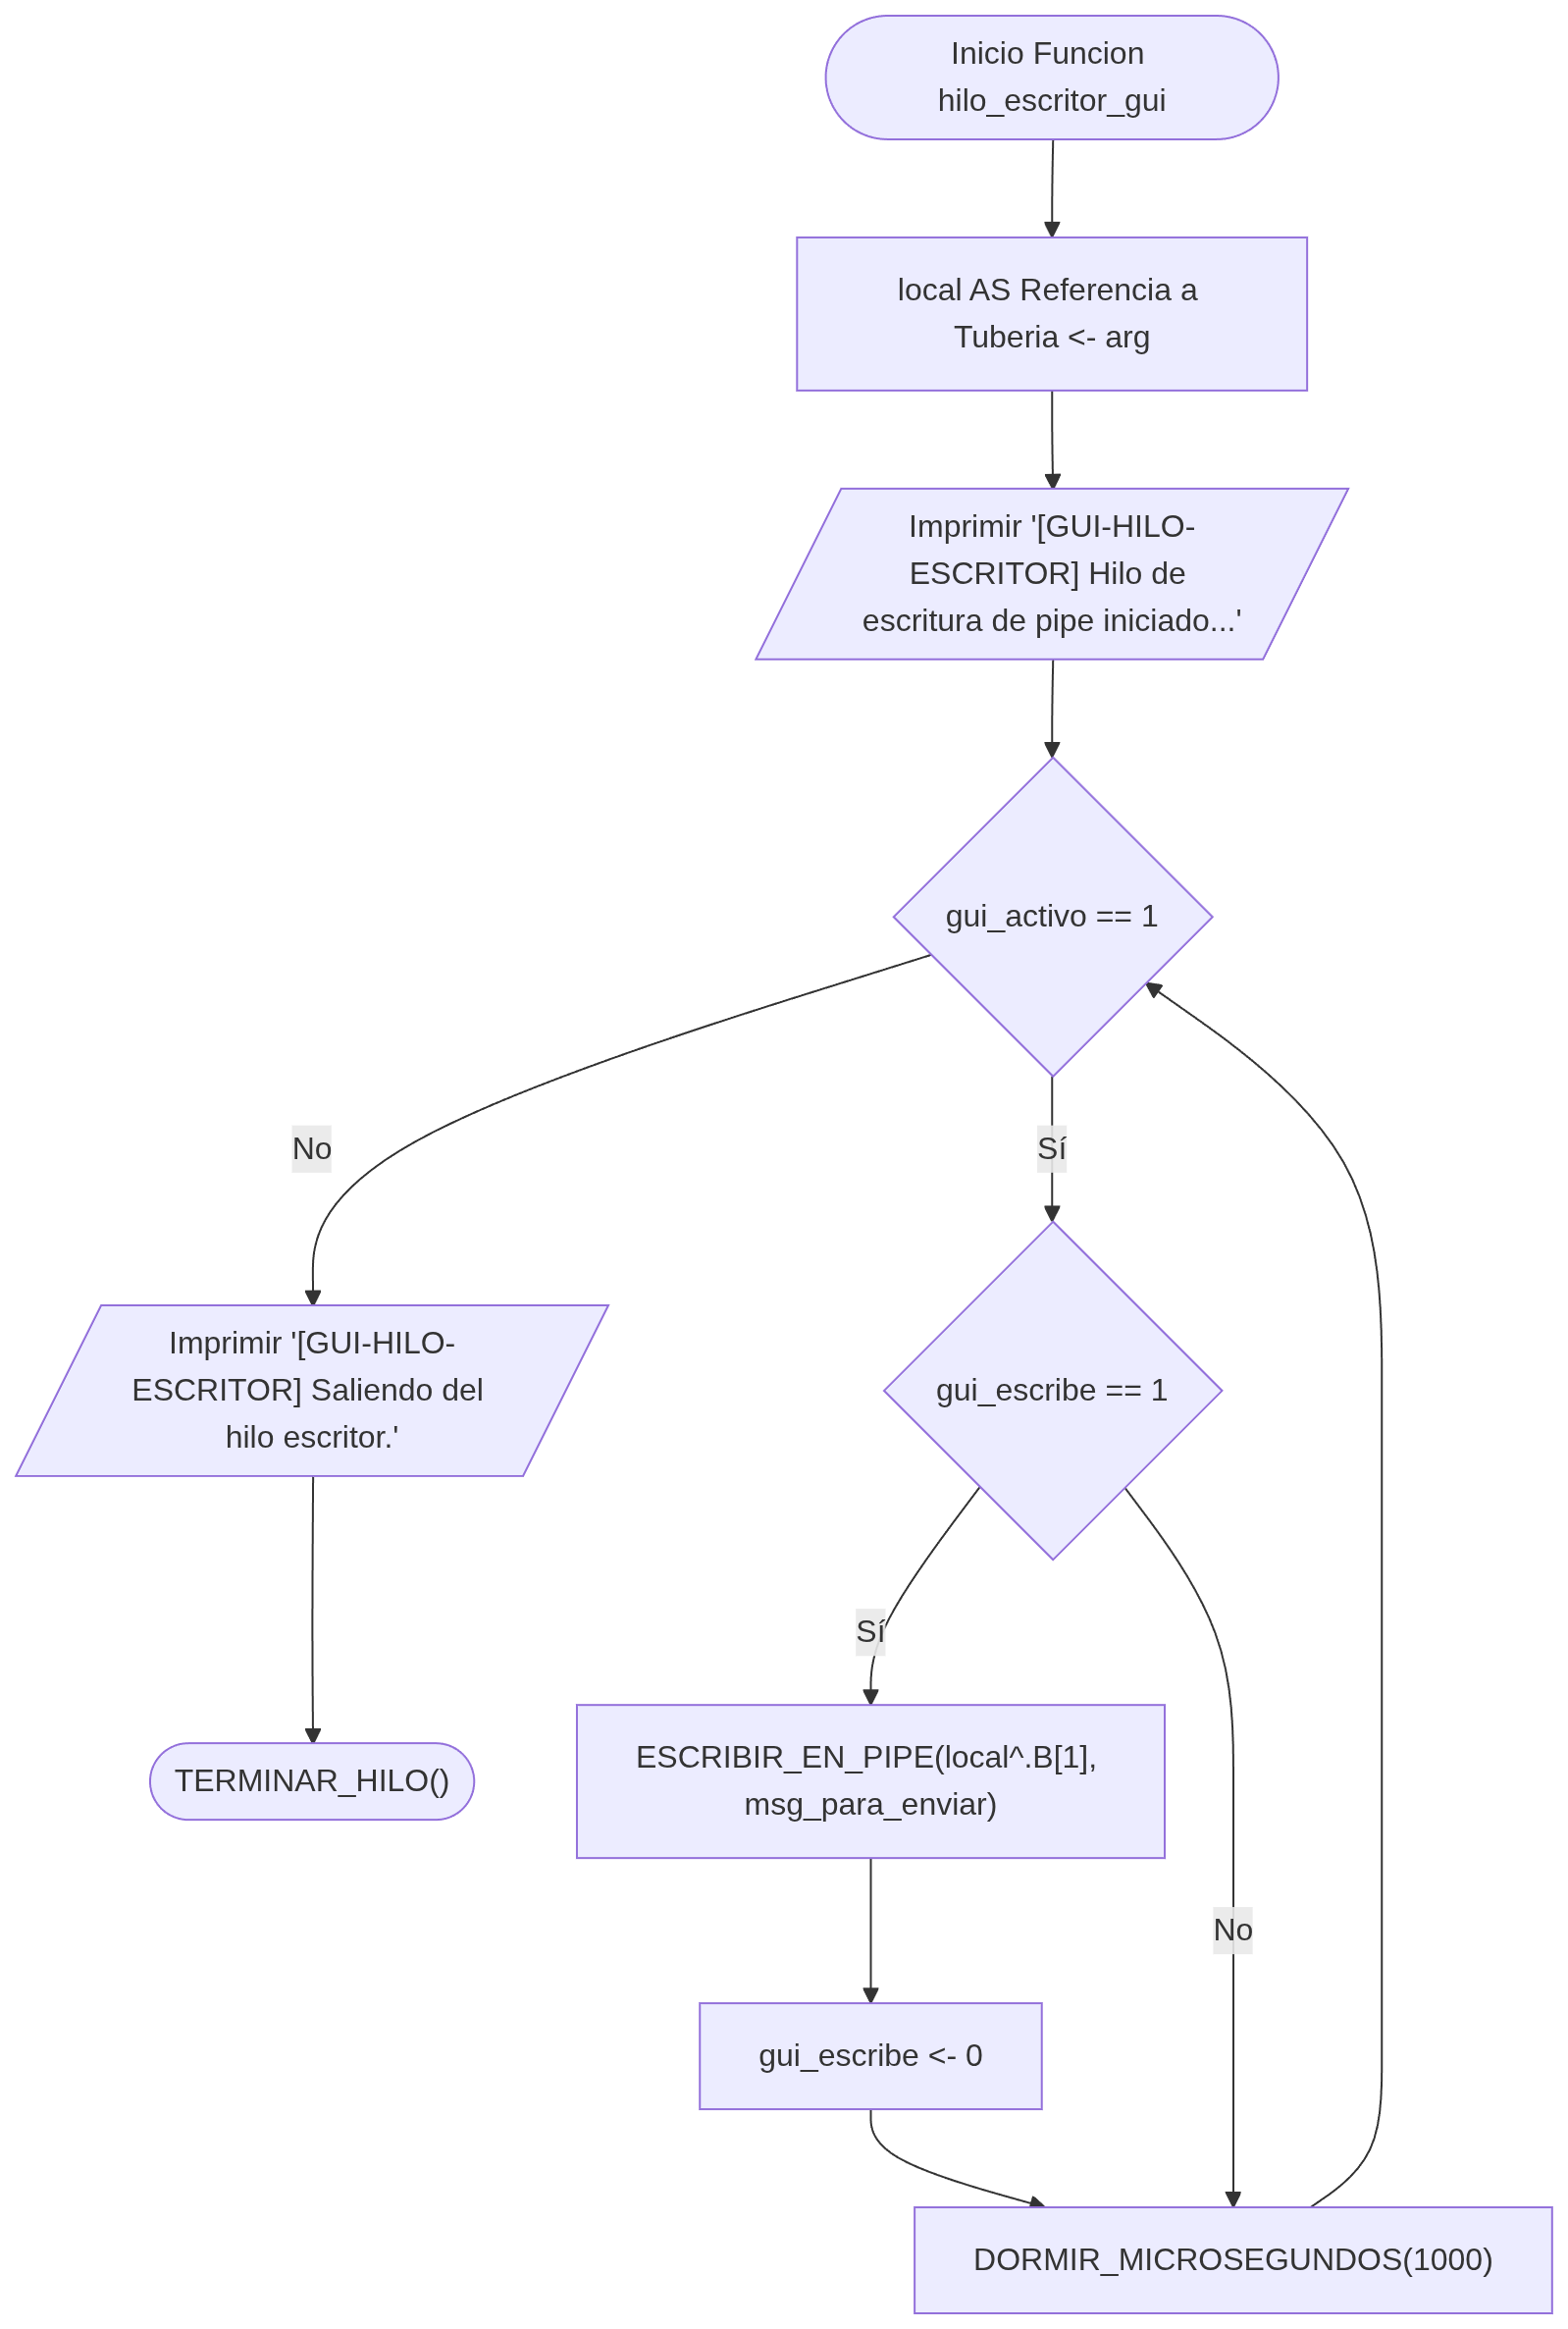
\includegraphics[width=0.5\textwidth]{Diagramas3/hilo_escritor_gui.png} 
\end{figure}

% --- PROCEDIMIENTO 4 ---
\newpage
\paragraph{4. Procedimiento \texttt{añadir\_burbuja()}} ~\\
\begin{figure}[H]
    \centering
    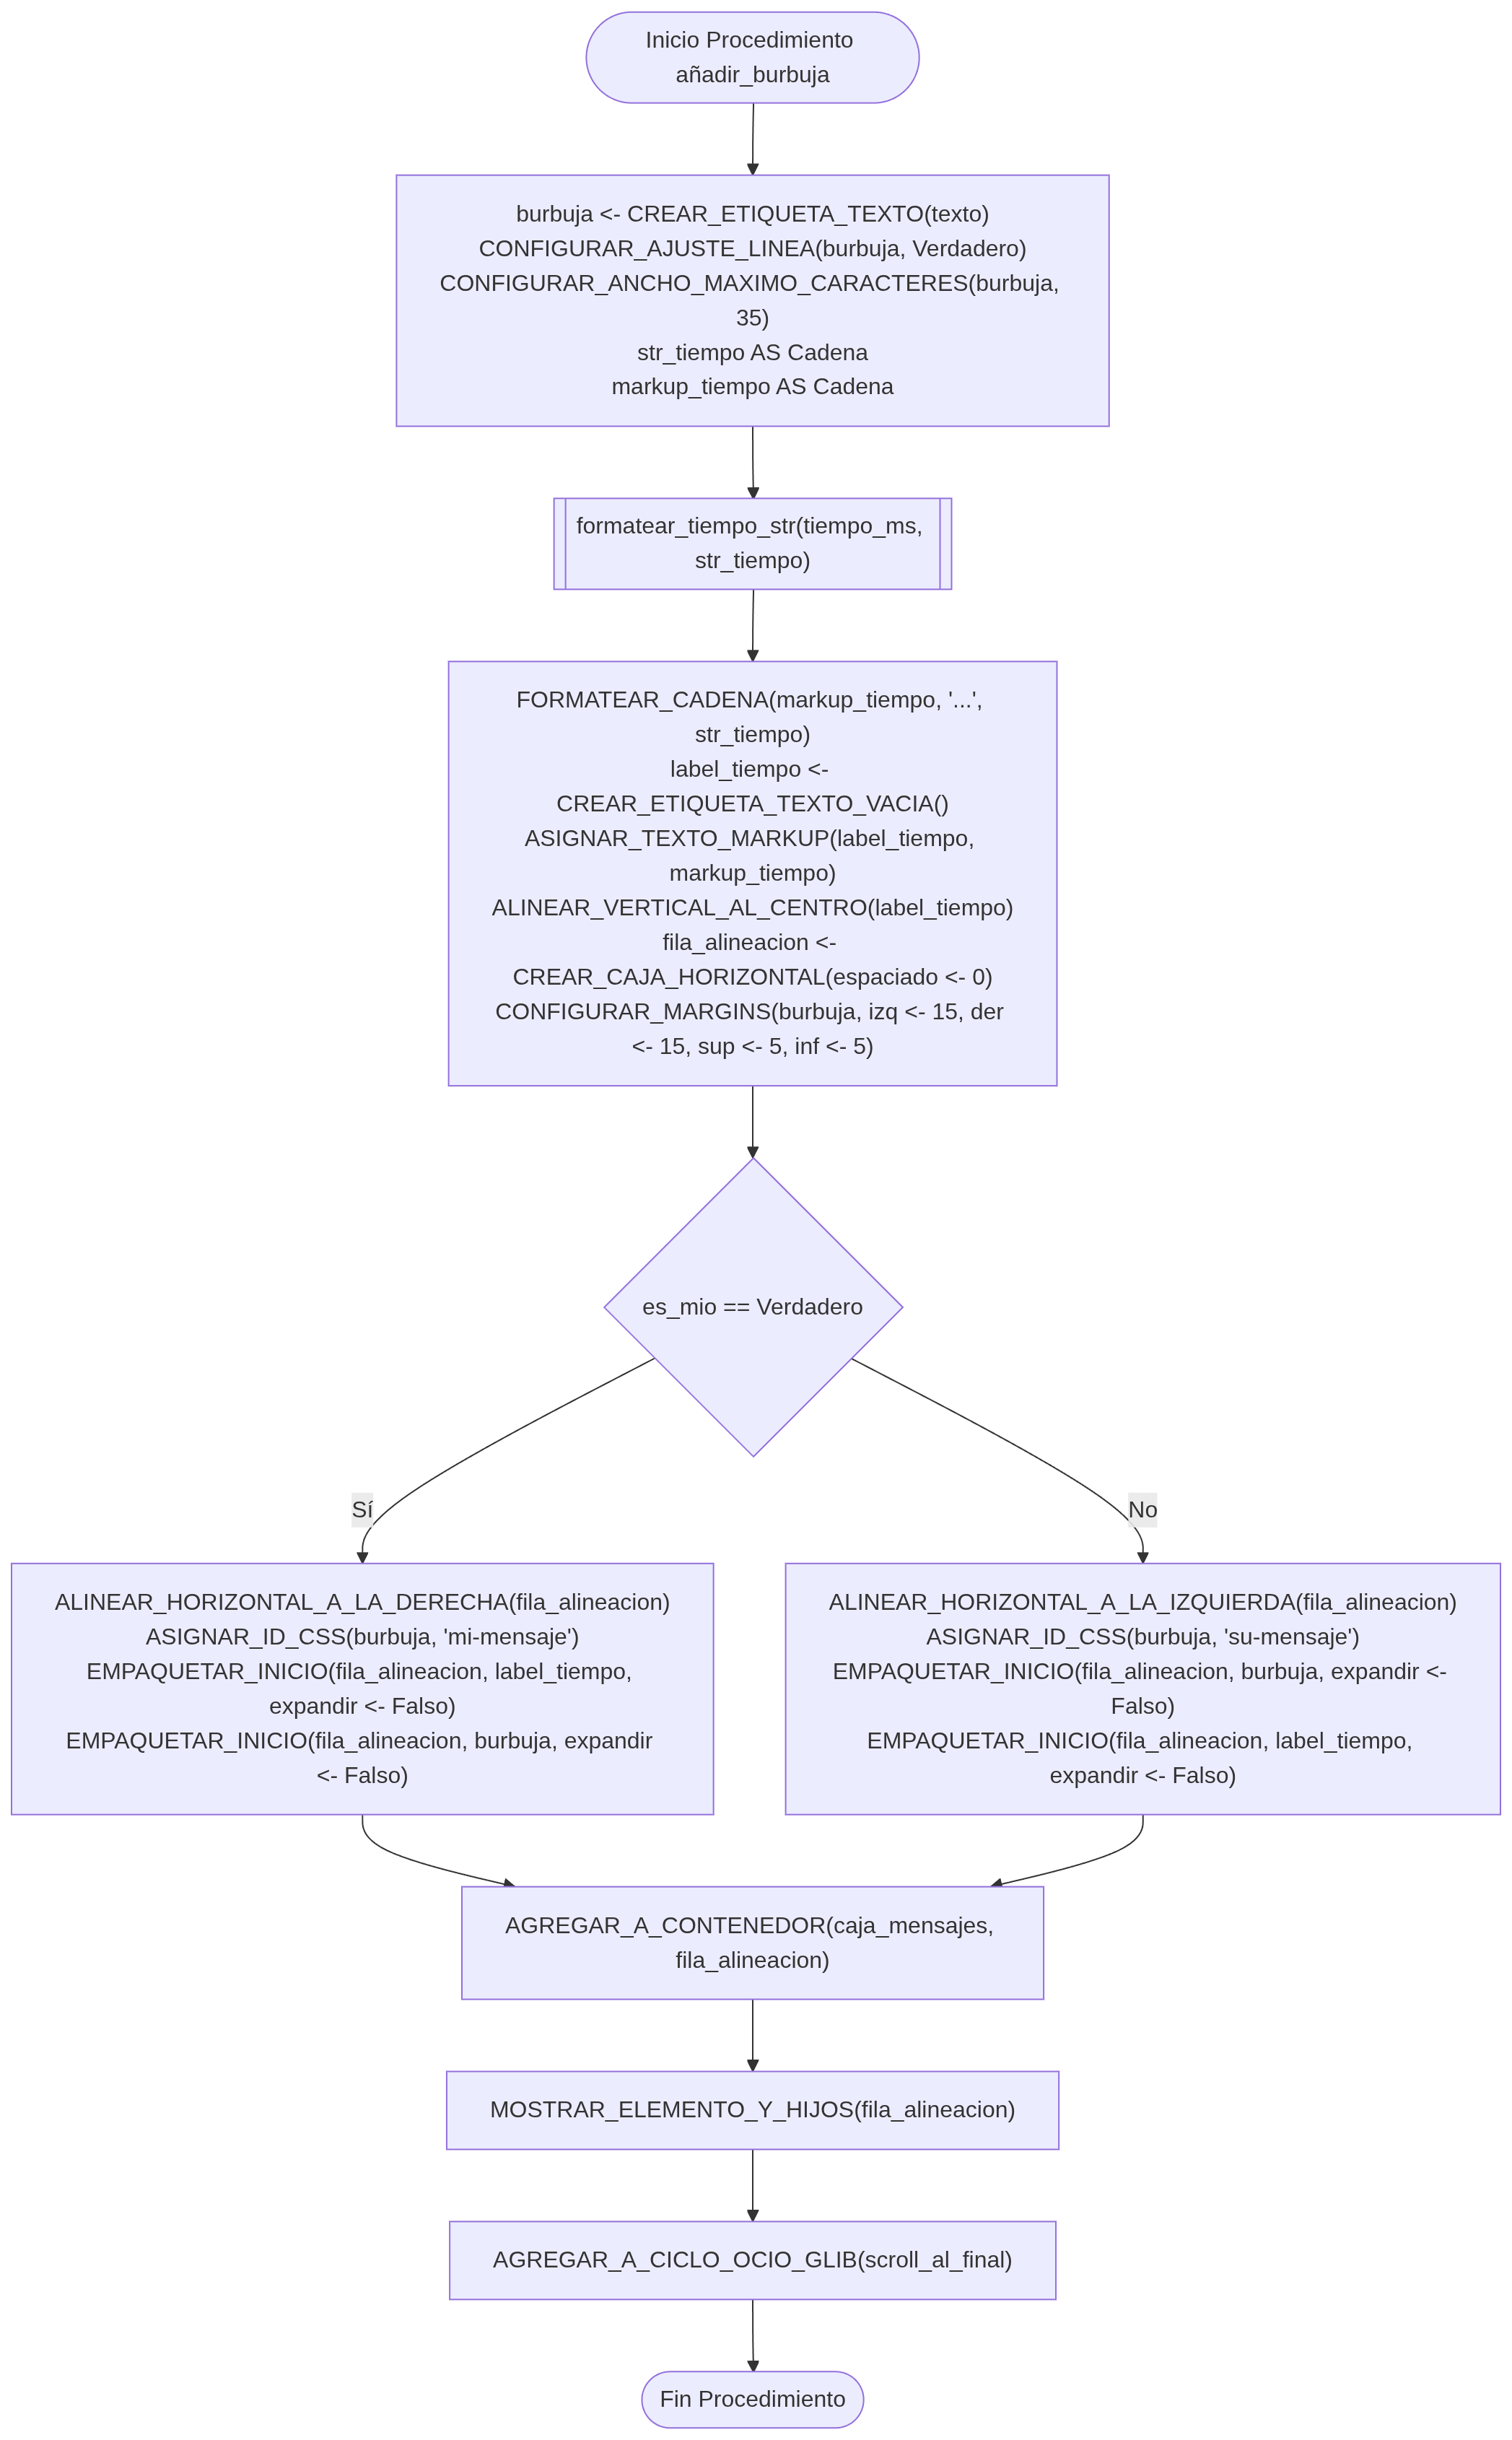
\includegraphics[width=0.6\textwidth]{Diagramas3/añadir_burbuja.png} 
\end{figure}

% --- PROCEDIMIENTO 5 ---
\newpage
\paragraph{5. Procedimiento \texttt{boton\_pulsado()}} ~\\
\begin{figure}[H]
    \centering
    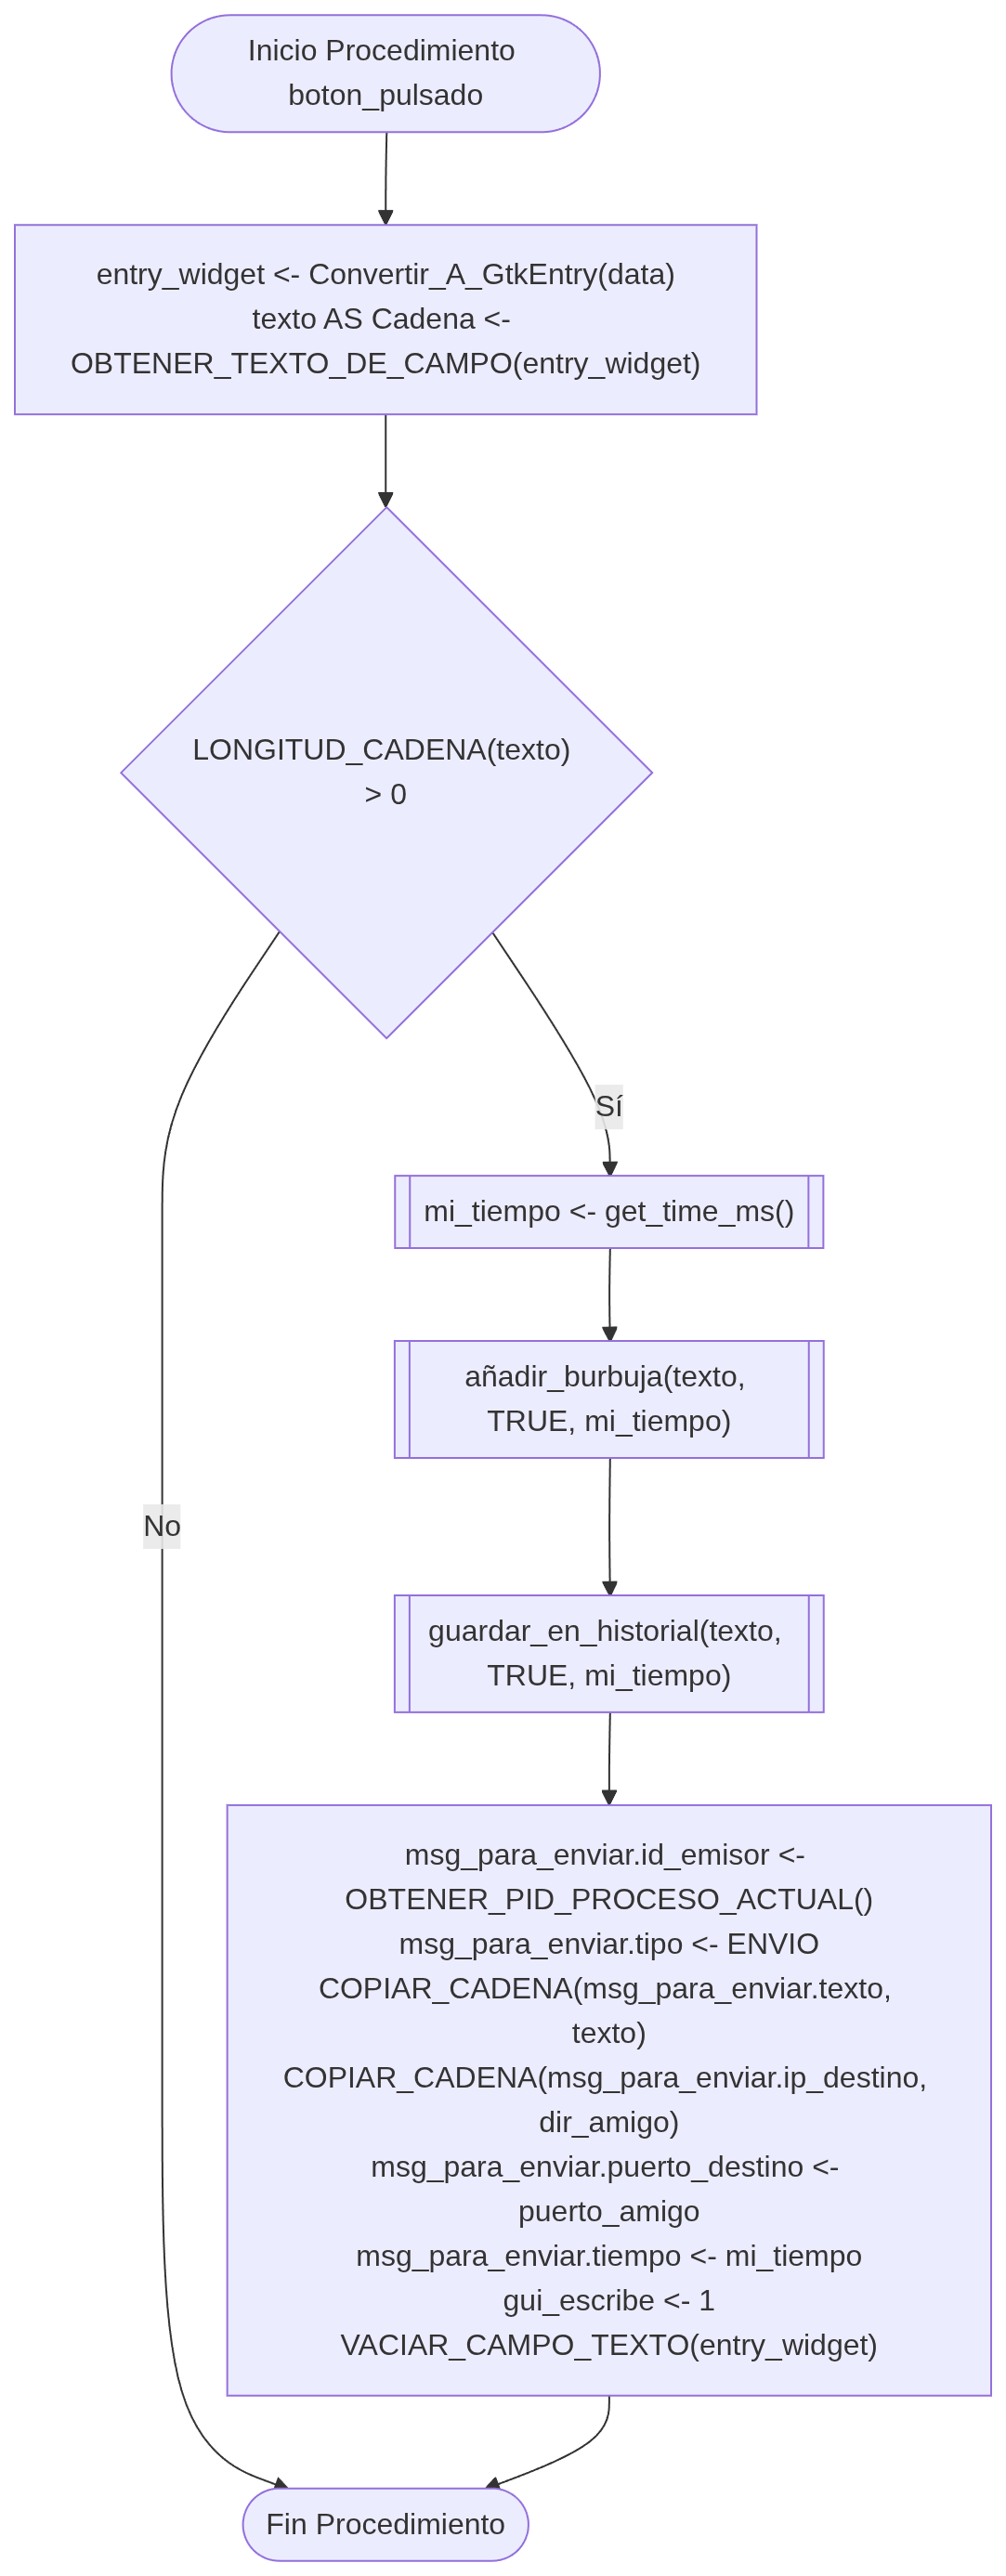
\includegraphics[width=0.4\textwidth]{Diagramas3/boton_pulsado.png} 
\end{figure}

% --- PROCEDIMIENTO 6 ---
\newpage
\paragraph{6. Procedimiento \texttt{ventana\_destruida()}} ~\\
\begin{figure}[H]
    \centering
    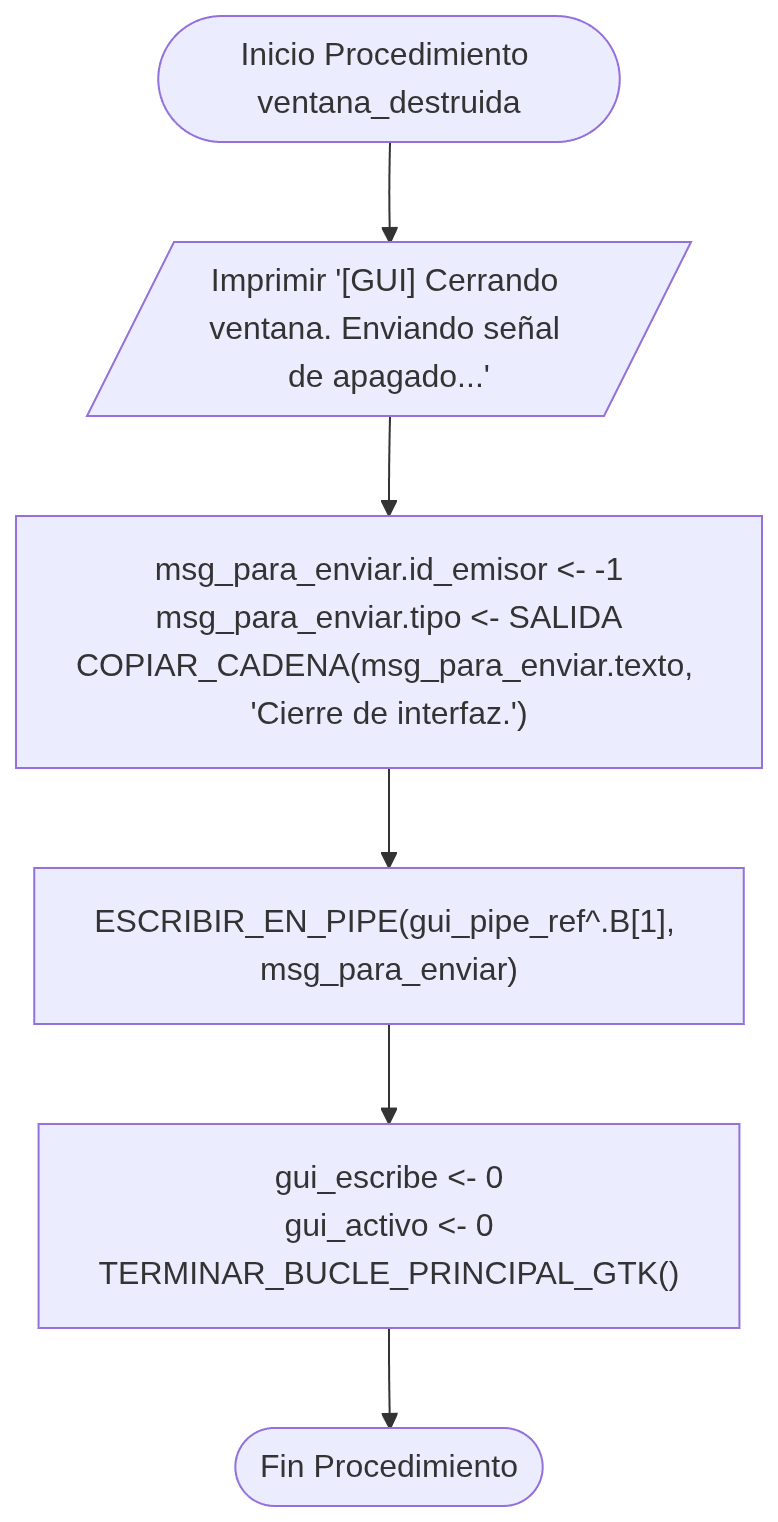
\includegraphics[width=0.4\textwidth]{Diagramas3/ventana_destruida.png} 
\end{figure}

% --- PROCEDIMIENTO 7 ---
\newpage
\paragraph{7. Procedimiento \texttt{guardar\_en\_historial()}} ~\\
\begin{figure}[H]
    \centering
    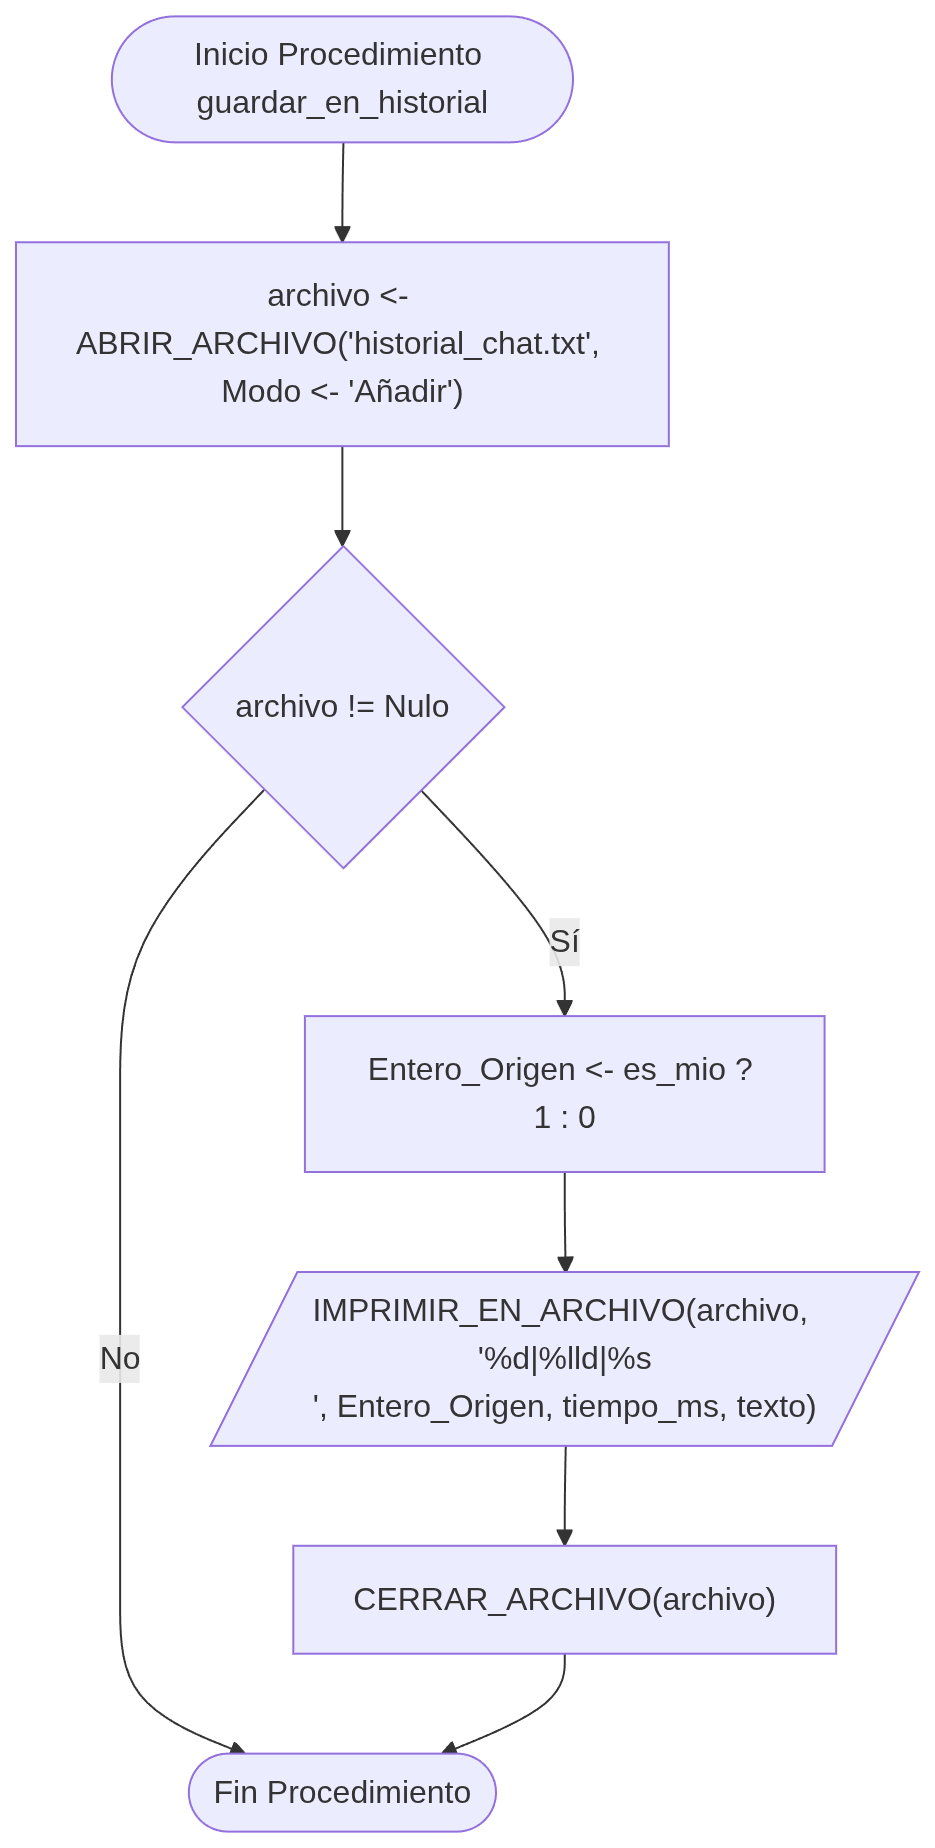
\includegraphics[width=0.4\textwidth]{Diagramas3/guardar_en_historial.png} 
\end{figure}

% --- PROCEDIMIENTO 8 ---
\newpage
\paragraph{8. Procedimiento \texttt{cargar\_historial()}} ~\\
\begin{figure}[H]
    \centering
    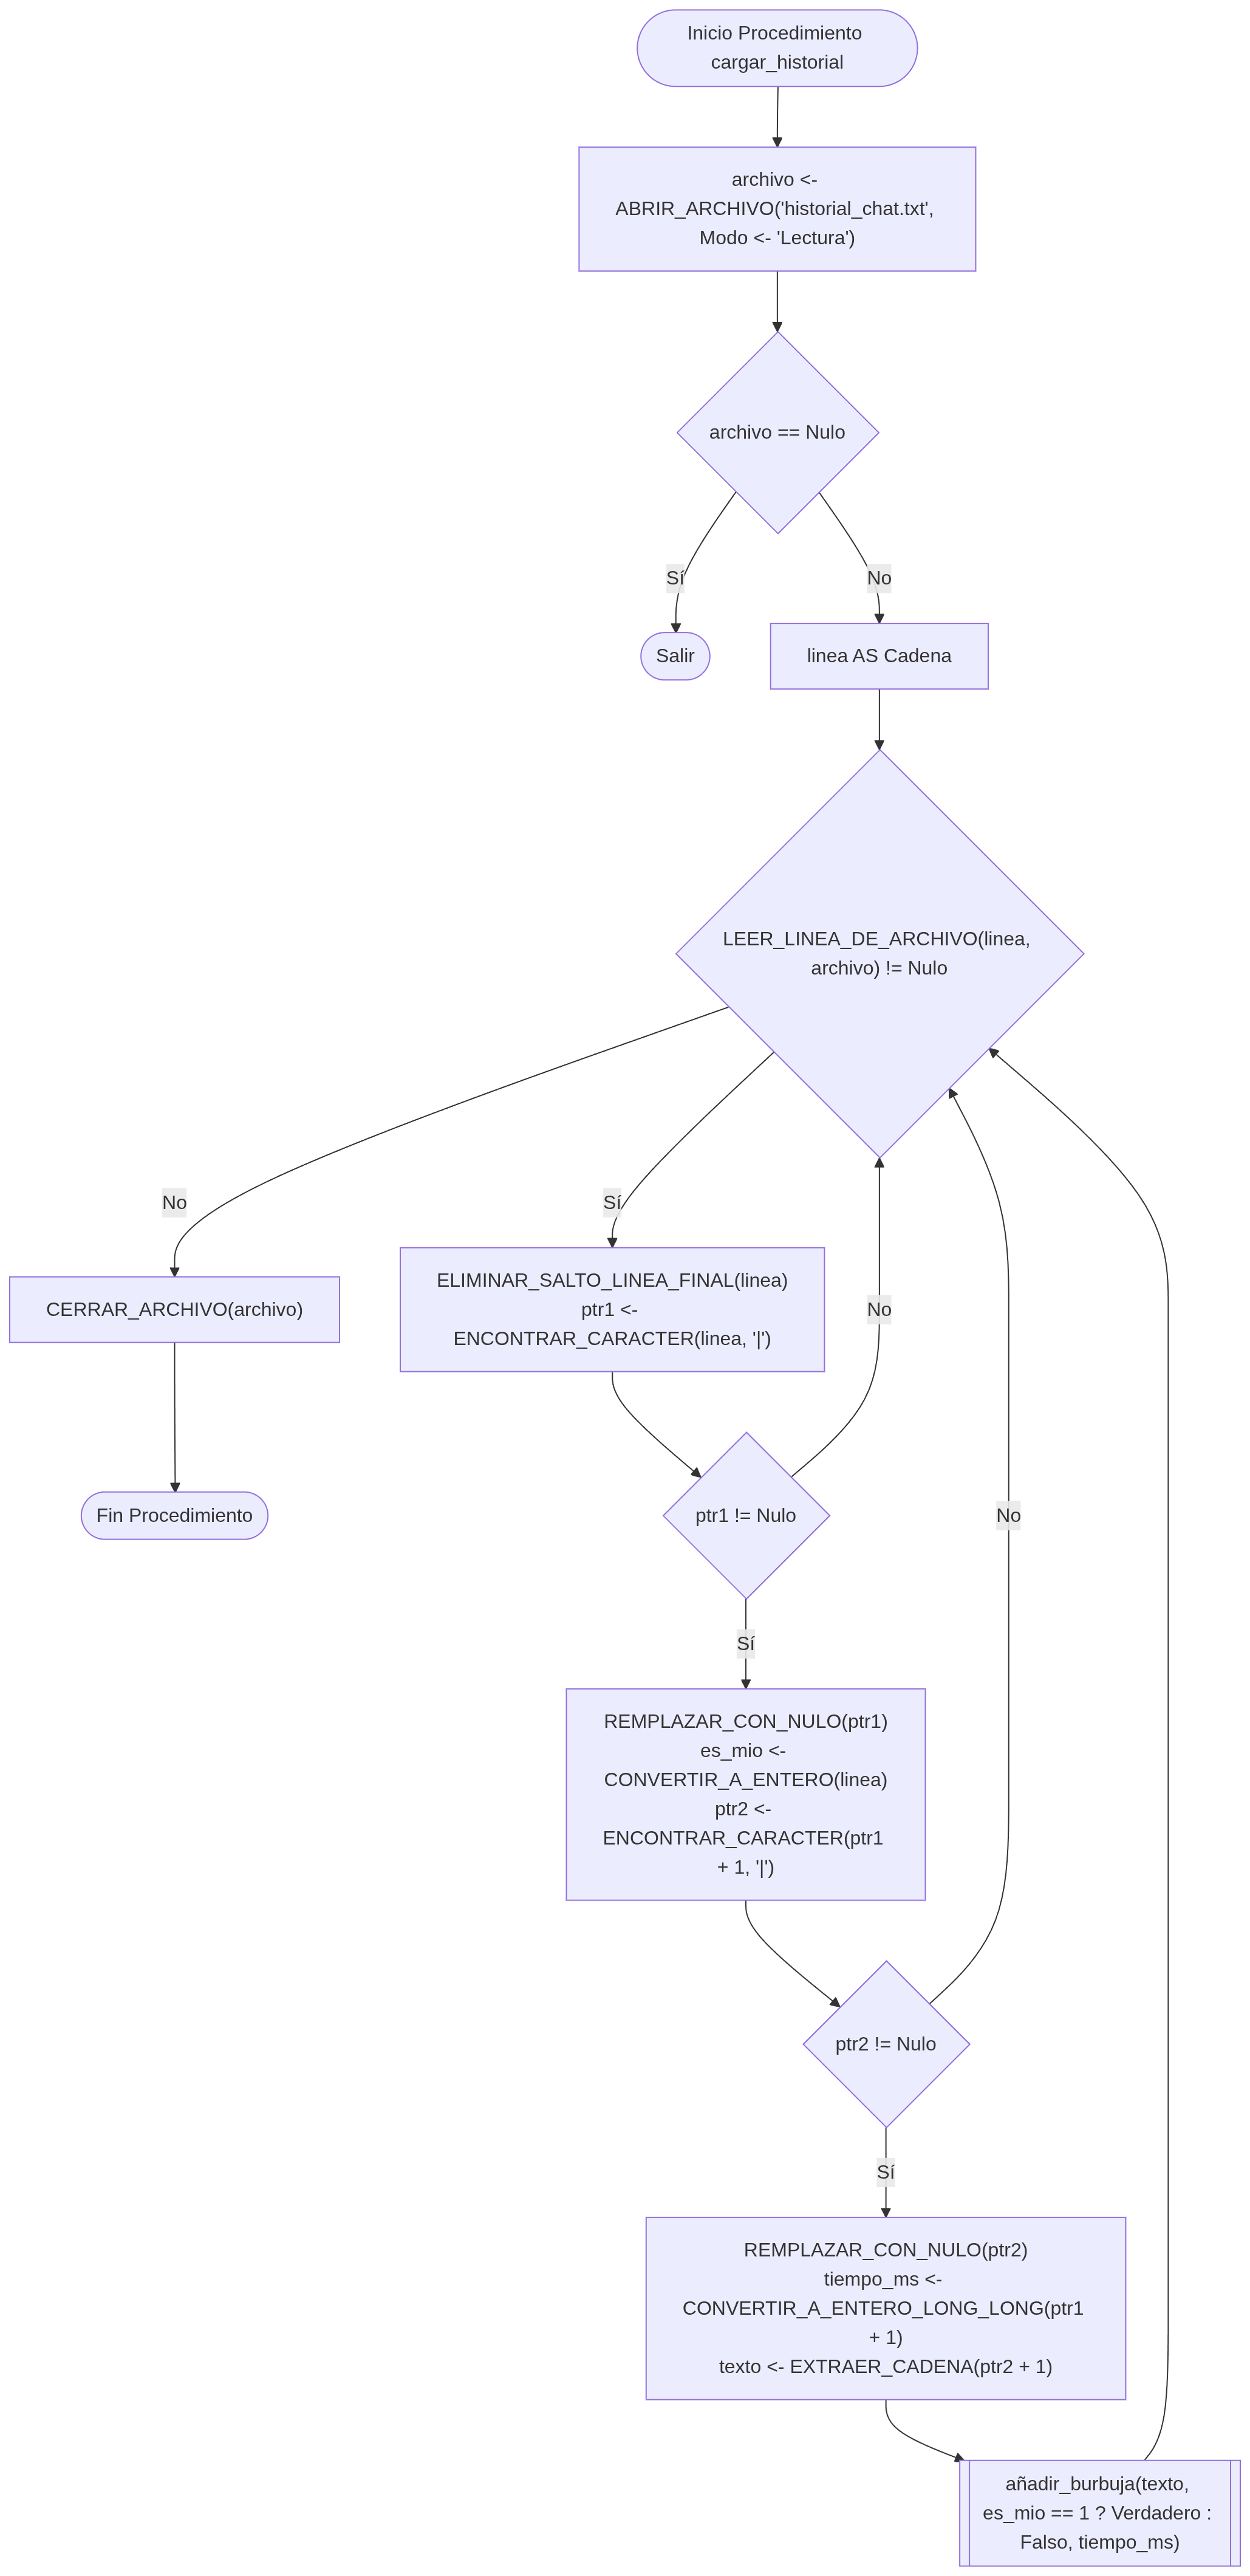
\includegraphics[width=0.5\textwidth]{Diagramas3/cargar_historial.png} 
\end{figure}

% --- PROCEDIMIENTO 9 ---
\newpage
\paragraph{9. Procedimiento \texttt{limpiar\_historial\_pulsado()}} ~\\
\begin{figure}[H]
    \centering
    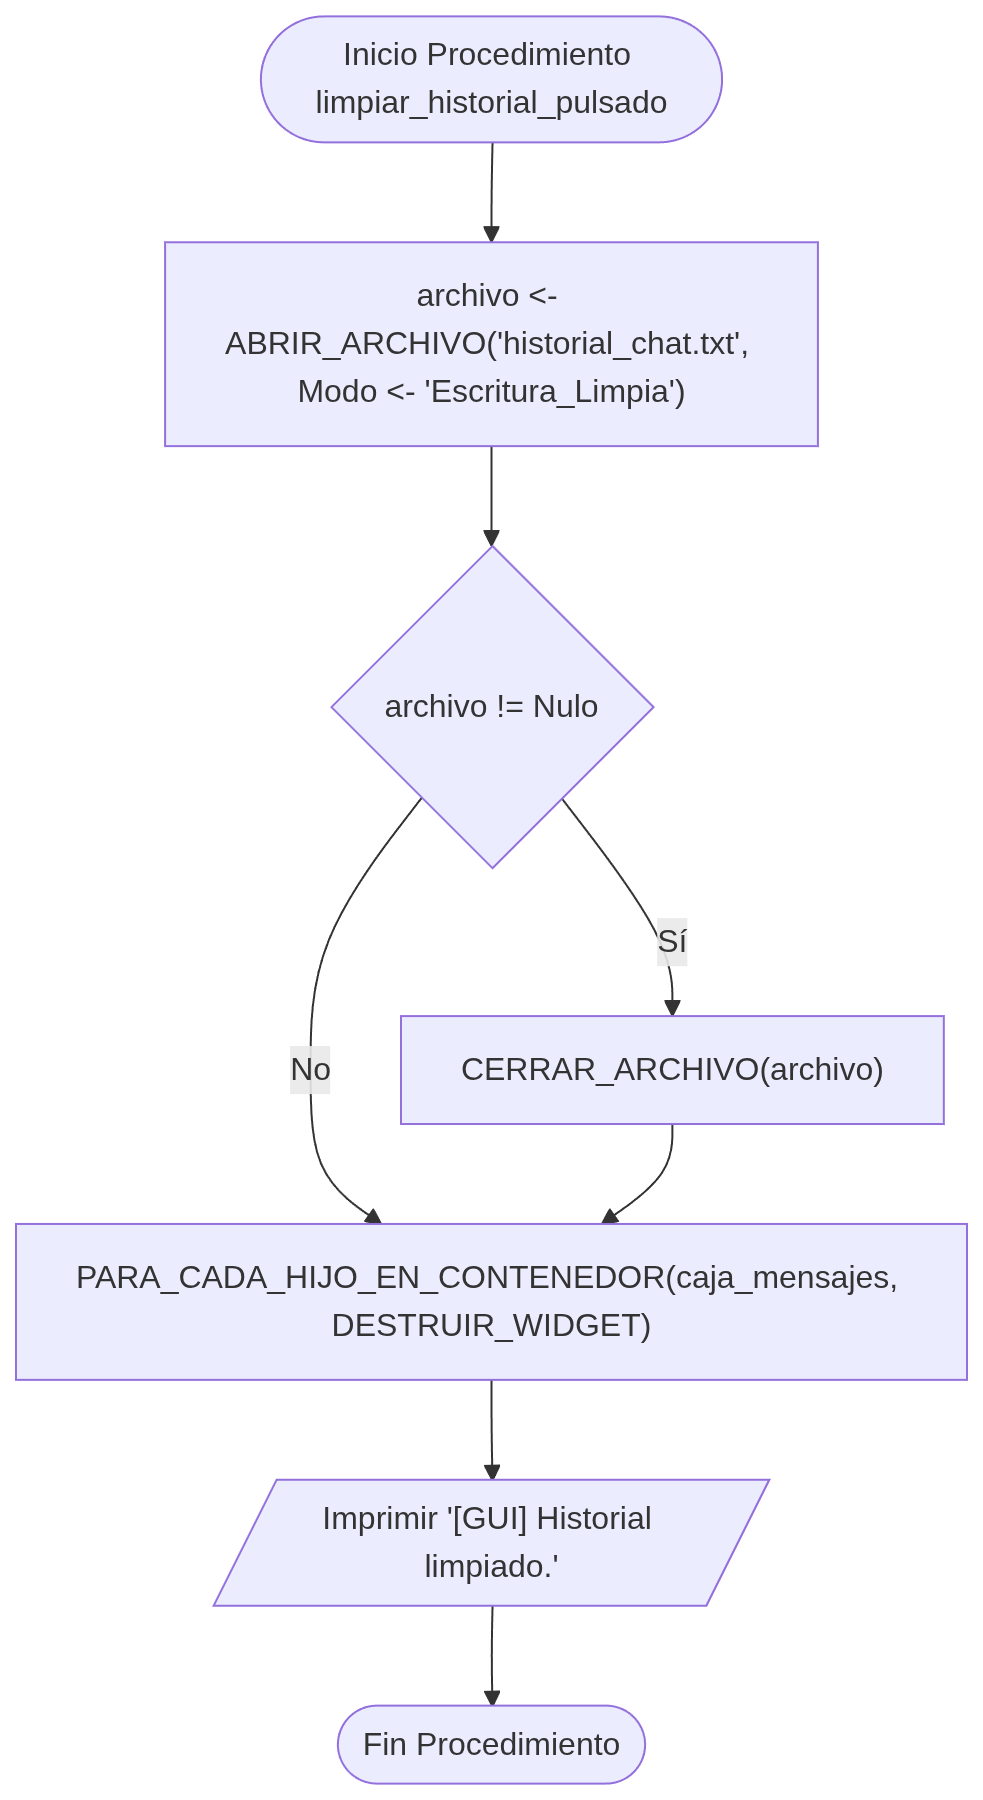
\includegraphics[width=0.4\textwidth]{Diagramas3/limpiar_historial_pulsado.png} 
\end{figure}

% --- FUNCION 10 ---
\newpage
\paragraph{10. Función \texttt{scroll\_al\_final()}} ~\\
\begin{figure}[H]
    \centering
    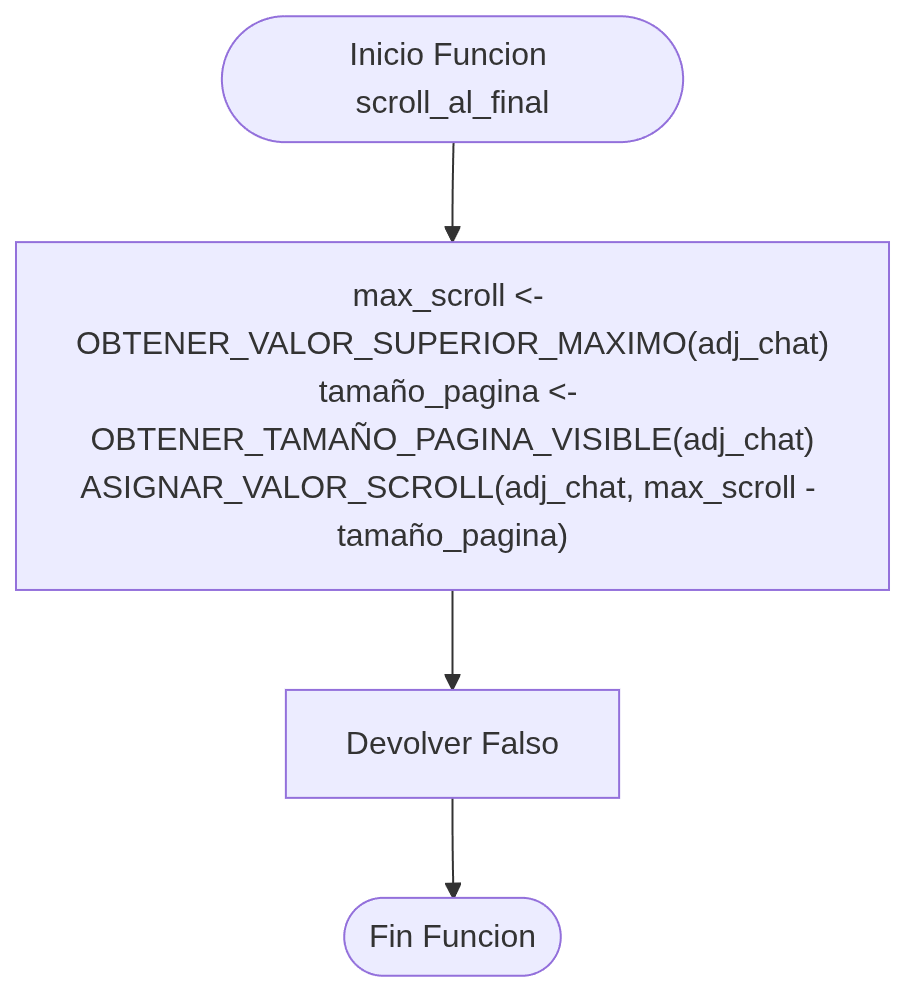
\includegraphics[width=0.4\textwidth]{Diagramas3/scroll_al_final.png} 
\end{figure}

% --- FUNCION 11 ---
\paragraph{11. Función \texttt{mostrar\_mensaje\_recibido()}} ~\\
\begin{figure}[H]
    \centering
    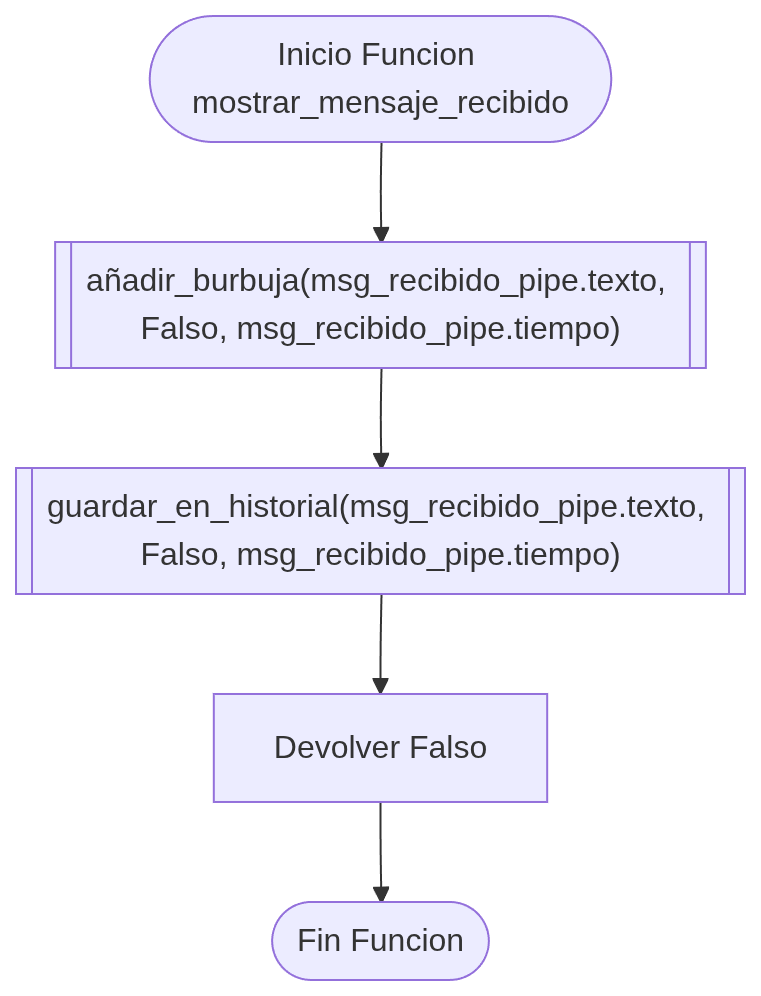
\includegraphics[width=0.4\textwidth]{Diagramas3/mostrar_mensaje_recibido.png} 
\end{figure}

% --- PROCEDIMIENTO 12 ---
\newpage
\paragraph{12. Procedimiento \texttt{cargar\_css()}} ~\\
\begin{figure}[H]
    \centering
    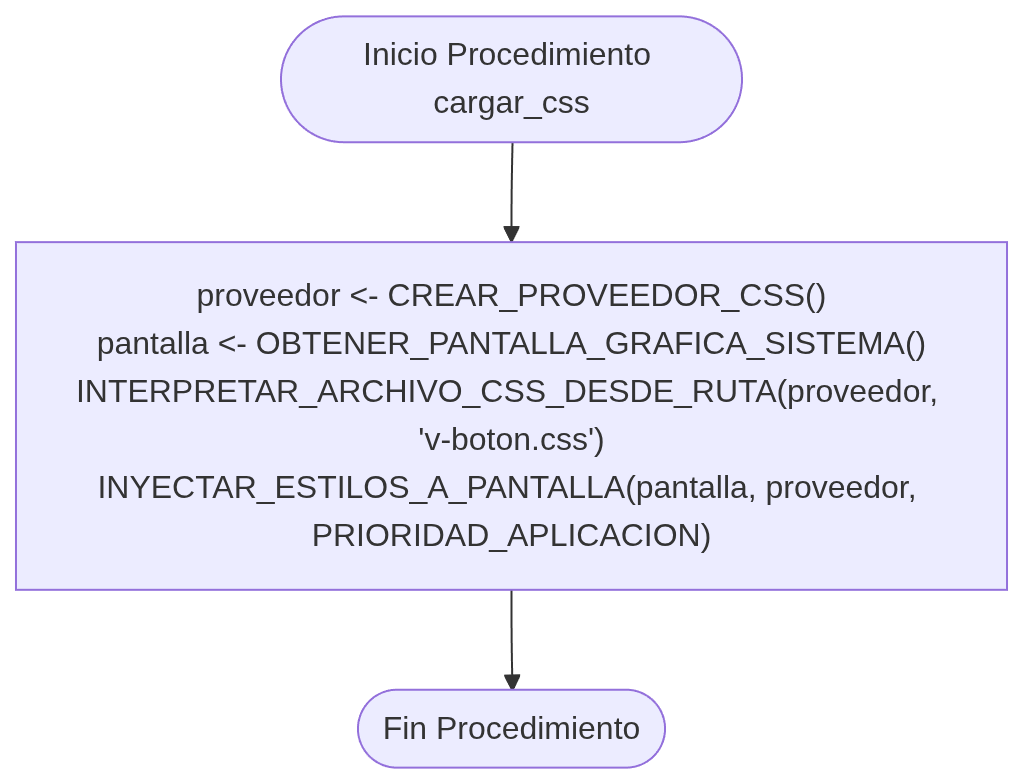
\includegraphics[width=0.4\textwidth]{Diagramas3/cargar_css.png} 
\end{figure}
\subsection{\large Archivo Principal \texttt{(chat.c)}}
Este archivo es el orquestador de toda la lógica de la conexión P2P y la interfaz gráfica que se muestra al usuario. Al modular ambas partes, se requiere la bifurcación del sistema en dos procesos independientes (un padre y un hijo) mediante la directiva \texttt{fork()}, lo que permite manejar la aplicación completa de forma concurrente sin que la red bloquee la interfaz.

\begin{lstlisting}[style=estiloC]
#include <stdio.h>
#include <stdlib.h>
#include <unistd.h>
#include <sys/wait.h>
#include "header.h"

// Tubería que se usa para comunicar los dos procesos (Pipe A y Pipe B)
Tuberia principal;

int main(int argc, char *argv[])
{
    // Creamos las dos tuberías a utilizar durante la ejecución
    if (pipe(principal.B) < 0 || pipe(principal.A) < 0)
    {
        perror("Error al crear los pipes");
        return 1;
    }
    
    // Creamos un proceso hijo mediante fork para levantar la conexión P2P
    pid_t process = fork();
    
    // Si ocurre algún error en la bifurcación, se cancela la ejecución
    if (process < 0)
        return 1;
        
    // De lo contrario, el proceso hijo (process == 0) se encarga de la conexión P2P
    if (process == 0)
    {
        // El hijo cierra los extremos no usados de las tuberías
        close(principal.A[0]);
        close(principal.B[1]);
        
        // Llama a la función que levanta la red y los sockets
        conexion(&principal);
        
        // Cierra los extremos utilizados para terminar exitosamente y liberar memoria
        close(principal.A[1]); 
        close(principal.B[0]);

        exit(0);
    }
    else // El proceso padre se encarga de renderizar la interfaz gráfica
    {
        // Se duerme 2 segundos para dar tiempo a que el back-end levante el servidor
        sleep(2);
        
        // El padre cierra los extremos que no utiliza de las tuberías
        close(principal.A[1]);
        close(principal.B[0]);
        
        // Llama a la función principal de GTK que crea la vista
        interfaz_grafica(argc, argv, &principal);
        
        // Cierra los extremos utilizados tras cerrar la ventana
        close(principal.A[0]); 
        close(principal.B[1]);
        
        // El padre espera a que el proceso hijo termine para cerrarse exitosamente
        wait(NULL);
    }
    return 0;
}
\end{lstlisting}
\input{pseudocodigo4.tex}
% \subsubsection{\large Diagrama de flujo \texttt{(chat.c)}}



\subsection{\large Conexión Física y Enrutamiento de Red (Tailscale)}
Para establecer la comunicación peer to peer entre dos computadoras ubicadas en distintas redes geográficas, nos enfrentamos al problema clásico de las restricciones de red impuestas por los ruteadores y el NAT (\textit{Network Address Translation}) de los proveedores de servicios de internet (ISP), los cuales bloquean las conexiones entrantes por defecto.

Para resolver este desafío de conectividad sin necesidad de realizar configuraciones invasivas como el \textit{Port Forwarding} en cada módem, se implementó \textbf{Tailscale}. Esta herramienta es una VPN de malla (\textit{Mesh VPN}) basada en el protocolo WireGuard que crea una red privada virtual superpuesta. 

Al instalar Tailscale en ambas máquinas, el software les asigna una dirección IP estática dentro de una misma subred virtual (por ejemplo, en el rango \texttt{100.x.x.x}). Esto permite que los \textit{sockets} de nuestra aplicación en C puedan realizar el \texttt{bind()} y el \texttt{connect()} apuntando directamente a las direcciones IP virtuales proporcionadas por la plataforma, engañando al sistema para que interactúe como si ambas computadoras estuvieran conectadas al mismo conmutador (\textit{switch}) en una red de área local (LAN). De este modo, garantizamos un túnel encriptado, directo y de baja latencia para la transmisión de las estructuras \texttt{Mensaje}.

\newpage
\section{\large Conclusión}
\begin{itemize}
    \item \textbf{Enrique Yoab Cortez Rios}
\end{itemize}
El desarrollo de esta práctica representó un gran reto técnico, ya que la aplicación pasó por múltiples etapas de rectificación y optimización de recursos. La implementación de tuberías cruzadas (pipes) y la asignación de hilos específicos para la lectura y escritura entre el front-end y el back-end resultó ser la solución más eficiente. Esta arquitectura nos permitió comunicar los procesos de forma directa y asíncrona, evitando el uso de intermediarios para transferir los datos entre la red y la interfaz.

Por otro lado, la biblioteca GTK fue fundamental para construir una interfaz gráfica nativa íntegramente en C. Una gran ventaja de esta herramienta fue la posibilidad de estilizar la ventana mediante un archivo CSS. Al tener experiencia previa con el desarrollo web y la estructura de componentes visuales, integrar estas hojas de estilo resultó un proceso muy natural, permitiendo dotar al chat de una apariencia mucho más atractiva, moderna y amigable para el usuario.

Asimismo, la implementación de Tailscale fue un gran acierto para la arquitectura del proyecto, ya que nos permitió establecer una conexión peer-to-peer a través de internet, enlazando ambas computadoras mediante direcciones IP virtuales sin la estricta necesidad de estar conectadas físicamente por un cable Ethernet en la misma red local.

En conclusión, la práctica se completó con éxito y cumplió sus objetivos formativos. Se consolidaron los conceptos de programación concurrente, logrando distribuir la carga de trabajo entre los procesos para mantener todo el sistema coordinado. El uso de hilos (pthreads) demostró ser clave para manejar las operaciones bloqueantes de escucha y escritura en las tuberías y los sockets, garantizando que la interfaz gráfica se mantuviera reactiva en todo momento y libre de congelamientos.


\section{\large Referencias}
\begin{itemize}
    \item Oporto Díaz, S. (s.f.). Material Adicional (SOSD – Mod 4): Concurrencia. Exclusión mutua y sincronización [PDF]. Departamento de Ciencias e Ingeniería de la Computación, Universidad Nacional del Sur. Disponible en \href{https://cs.uns.edu.ar/~gd/soyd/clases/04-SincronizacionExtras.pdf}{cs.uns.edu.ar}.
    
    \item De Luz, S. (2026, 12 marzo). Tailscale, conecta equipos a una red privada virtual (VPN) fácilmente. RedesZone. Disponible en \href{https://www.redeszone.net/tutoriales/vpn/configurar-tailscale-red-vpn-segura/}{RedesZone}.
    
    \item Purita, G. (2026, 17 marzo). ¿Qué son las redes P2P y cuál su utilidad? OBS Business School. Disponible en \href{https://www.obsbusiness.school/blog/que-son-las-redes-p2p-y-cual-su-utilidad}{OBS Business School}.
    
    \item Hilo en computación: ¿Qué es? | Lenovo México. (s. f.). Disponible en \href{https://www.lenovo.com/mx/es/glosario/hilo/?orgRef=https%253A%252F%252Fwww.google.com%252F}{Lenovo México}.
    
    \item Klie, F. R. (2026, 5 marzo). Understanding `fork()` in Linux: How Process Creation Really Works. DEV Community. Disponible en \href{https://dev-to.translate.goog/farhadrahimiklie/understanding-fork-in-linux-how-process-creation-really-works-13id?_x_tr_sl=en&_x_tr_tl=es&_x_tr_hl=es&_x_tr_pto=sge}{DEV Community}.
    \item Team, G. (s. f.). The GTK Project - A free and open-source cross-platform widget toolkit. The GTK Team. \href{https://www.gtk.org/}{Web oficial GTK}
\end{itemize}

\end{document}